\documentclass[1p]{elsarticle_modified}
%\bibliographystyle{elsarticle-num}

%\usepackage[colorlinks]{hyperref}
%\usepackage{abbrmath_seonhwa} %\Abb, \Ascr, \Acal ,\Abf, \Afrak
\usepackage{amsfonts}
\usepackage{amssymb}
\usepackage{amsmath}
\usepackage{amsthm}
\usepackage{scalefnt}
\usepackage{amsbsy}
\usepackage{kotex}
\usepackage{caption}
\usepackage{subfig}
\usepackage{color}
\usepackage{graphicx}
\usepackage{xcolor} %% white, black, red, green, blue, cyan, magenta, yellow
\usepackage{float}
\usepackage{setspace}
\usepackage{hyperref}

\usepackage{tikz}
\usetikzlibrary{arrows}

\usepackage{multirow}
\usepackage{array} % fixed length table
\usepackage{hhline}

%%%%%%%%%%%%%%%%%%%%%
\makeatletter
\renewcommand*\env@matrix[1][\arraystretch]{%
	\edef\arraystretch{#1}%
	\hskip -\arraycolsep
	\let\@ifnextchar\new@ifnextchar
	\array{*\c@MaxMatrixCols c}}
\makeatother %https://tex.stackexchange.com/questions/14071/how-can-i-increase-the-line-spacing-in-a-matrix
%%%%%%%%%%%%%%%

\usepackage[normalem]{ulem}

\newcommand{\msout}[1]{\ifmmode\text{\sout{\ensuremath{#1}}}\else\sout{#1}\fi}
%SOURCE: \msout is \stkout macro in https://tex.stackexchange.com/questions/20609/strikeout-in-math-mode

\newcommand{\cancel}[1]{
	\ifmmode
	{\color{red}\msout{#1}}
	\else
	{\color{red}\sout{#1}}
	\fi
}

\newcommand{\add}[1]{
	{\color{blue}\uwave{#1}}
}

\newcommand{\replace}[2]{
	\ifmmode
	{\color{red}\msout{#1}}{\color{blue}\uwave{#2}}
	\else
	{\color{red}\sout{#1}}{\color{blue}\uwave{#2}}
	\fi
}

\newcommand{\Sol}{\mathcal{S}} %segment
\newcommand{\D}{D} %diagram
\newcommand{\A}{\mathcal{A}} %arc


%%%%%%%%%%%%%%%%%%%%%%%%%%%%%5 test

\def\sl{\operatorname{\textup{SL}}(2,\Cbb)}
\def\psl{\operatorname{\textup{PSL}}(2,\Cbb)}
\def\quan{\mkern 1mu \triangleright \mkern 1mu}

\theoremstyle{definition}
\newtheorem{thm}{Theorem}[section]
\newtheorem{prop}[thm]{Proposition}
\newtheorem{lem}[thm]{Lemma}
\newtheorem{ques}[thm]{Question}
\newtheorem{cor}[thm]{Corollary}
\newtheorem{defn}[thm]{Definition}
\newtheorem{exam}[thm]{Example}
\newtheorem{rmk}[thm]{Remark}
\newtheorem{alg}[thm]{Algorithm}

\newcommand{\I}{\sqrt{-1}}
\begin{document}

%\begin{frontmatter}
%
%\title{Boundary parabolic representations of knots up to 8 crossings}
%
%%% Group authors per affiliation:
%\author{Yunhi Cho} 
%\address{Department of Mathematics, University of Seoul, Seoul, Korea}
%\ead{yhcho@uos.ac.kr}
%
%
%\author{Seonhwa Kim} %\fnref{s_kim}}
%\address{Center for Geometry and Physics, Institute for Basic Science, Pohang, 37673, Korea}
%\ead{ryeona17@ibs.re.kr}
%
%\author{Hyuk Kim}
%\address{Department of Mathematical Sciences, Seoul National University, Seoul 08826, Korea}
%\ead{hyukkim@snu.ac.kr}
%
%\author{Seokbeom Yoon}
%\address{Department of Mathematical Sciences, Seoul National University, Seoul, 08826,  Korea}
%\ead{sbyoon15@snu.ac.kr}
%
%\begin{abstract}
%We find all boundary parabolic representation of knots up to 8 crossings.
%
%\end{abstract}
%\begin{keyword}
%    \MSC[2010] 57M25 
%\end{keyword}
%
%\end{frontmatter}

%\linenumbers
%\tableofcontents
%
\newcommand\colored[1]{\textcolor{white}{\rule[-0.35ex]{0.8em}{1.4ex}}\kern-0.8em\color{red} #1}%
%\newcommand\colored[1]{\textcolor{white}{ #1}\kern-2.17ex	\textcolor{white}{ #1}\kern-1.81ex	\textcolor{white}{ #1}\kern-2.15ex\color{red}#1	}

{\Large $\underline{12a_{0264}~(K12a_{0264})}$}

\setlength{\tabcolsep}{10pt}
\renewcommand{\arraystretch}{1.6}
\vspace{1cm}\begin{tabular}{m{100pt}>{\centering\arraybackslash}m{274pt}}
\multirow{5}{120pt}{
	\centering
	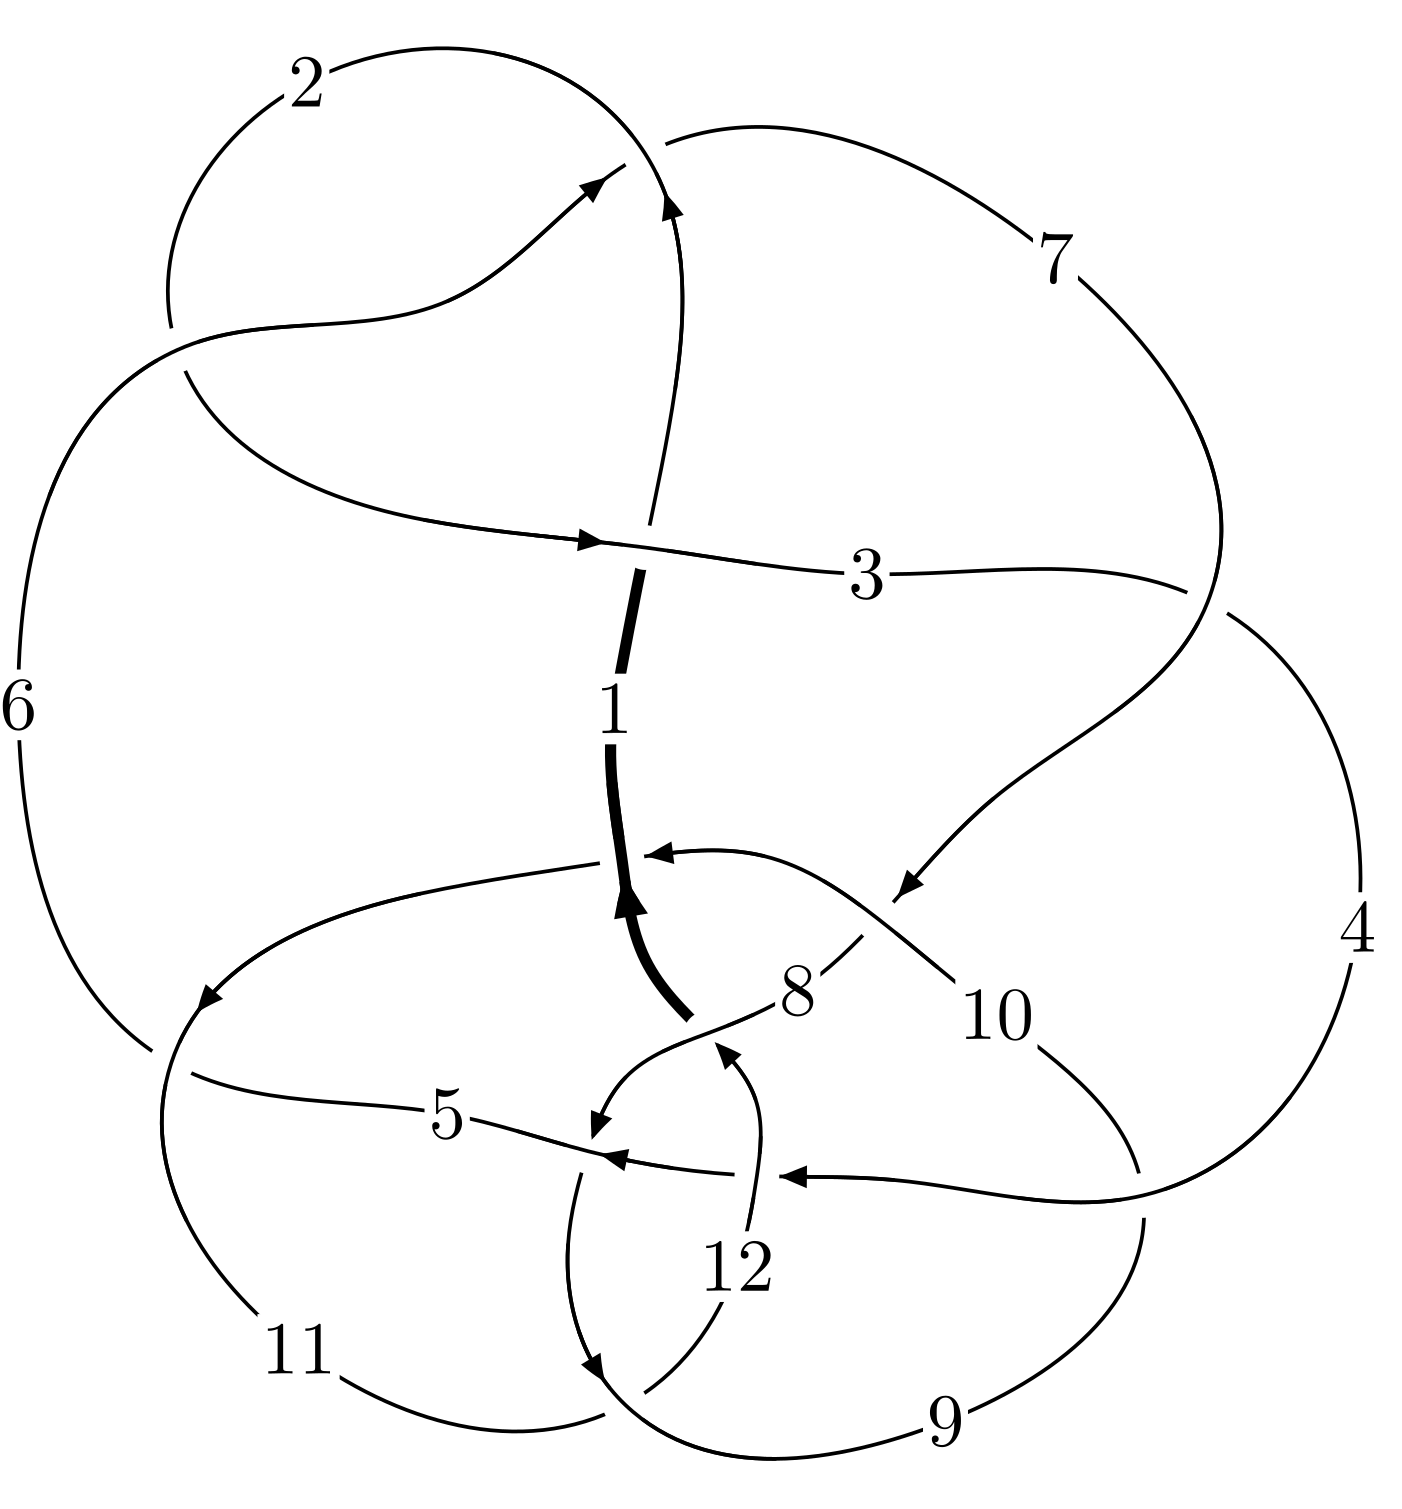
\includegraphics[width=112pt]{../../../GIT/diagram.site/Diagrams/png/1065_12a_0264.png}\\
\ \ \ A knot diagram\footnotemark}&
\allowdisplaybreaks
\textbf{Linearized knot diagam} \\
\cline{2-2}
 &
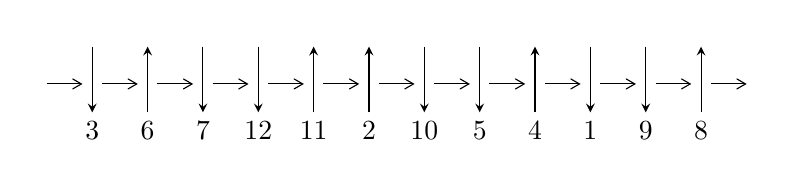
\begin{tikzpicture}[x=20pt, y=17pt]
	% nodes
	\node (C0) at (0, 0) {};
	\node (C1) at (1, 0) {};
	\node (C1U) at (1, +1) {};
	\node (C1D) at (1, -1) {3};

	\node (C2) at (2, 0) {};
	\node (C2U) at (2, +1) {};
	\node (C2D) at (2, -1) {6};

	\node (C3) at (3, 0) {};
	\node (C3U) at (3, +1) {};
	\node (C3D) at (3, -1) {7};

	\node (C4) at (4, 0) {};
	\node (C4U) at (4, +1) {};
	\node (C4D) at (4, -1) {12};

	\node (C5) at (5, 0) {};
	\node (C5U) at (5, +1) {};
	\node (C5D) at (5, -1) {11};

	\node (C6) at (6, 0) {};
	\node (C6U) at (6, +1) {};
	\node (C6D) at (6, -1) {2};

	\node (C7) at (7, 0) {};
	\node (C7U) at (7, +1) {};
	\node (C7D) at (7, -1) {10};

	\node (C8) at (8, 0) {};
	\node (C8U) at (8, +1) {};
	\node (C8D) at (8, -1) {5};

	\node (C9) at (9, 0) {};
	\node (C9U) at (9, +1) {};
	\node (C9D) at (9, -1) {4};

	\node (C10) at (10, 0) {};
	\node (C10U) at (10, +1) {};
	\node (C10D) at (10, -1) {1};

	\node (C11) at (11, 0) {};
	\node (C11U) at (11, +1) {};
	\node (C11D) at (11, -1) {9};

	\node (C12) at (12, 0) {};
	\node (C12U) at (12, +1) {};
	\node (C12D) at (12, -1) {8};
	\node (C13) at (13, 0) {};

	% arrows
	\draw[->,>={angle 60}]
	(C0) edge (C1) (C1) edge (C2) (C2) edge (C3) (C3) edge (C4) (C4) edge (C5) (C5) edge (C6) (C6) edge (C7) (C7) edge (C8) (C8) edge (C9) (C9) edge (C10) (C10) edge (C11) (C11) edge (C12) (C12) edge (C13) ;	\draw[->,>=stealth]
	(C1U) edge (C1D) (C2D) edge (C2U) (C3U) edge (C3D) (C4U) edge (C4D) (C5D) edge (C5U) (C6D) edge (C6U) (C7U) edge (C7D) (C8U) edge (C8D) (C9D) edge (C9U) (C10U) edge (C10D) (C11U) edge (C11D) (C12D) edge (C12U) ;
	\end{tikzpicture} \\
\hhline{~~} \\& 
\textbf{Solving Sequence} \\ \cline{2-2} 
 &
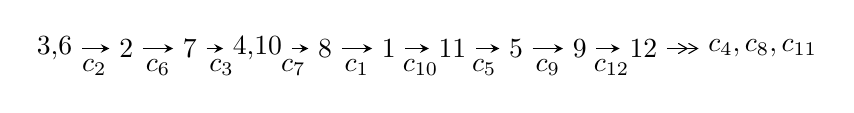
\begin{tikzpicture}[x=23pt, y=7pt]
	% node
	\node (A0) at (-1/8, 0) {3,6};
	\node (A1) at (1, 0) {2};
	\node (A2) at (2, 0) {7};
	\node (A3) at (49/16, 0) {4,10};
	\node (A4) at (33/8, 0) {8};
	\node (A5) at (41/8, 0) {1};
	\node (A6) at (49/8, 0) {11};
	\node (A7) at (57/8, 0) {5};
	\node (A8) at (65/8, 0) {9};
	\node (A9) at (73/8, 0) {12};
	\node (C1) at (1/2, -1) {$c_{2}$};
	\node (C2) at (3/2, -1) {$c_{6}$};
	\node (C3) at (5/2, -1) {$c_{3}$};
	\node (C4) at (29/8, -1) {$c_{7}$};
	\node (C5) at (37/8, -1) {$c_{1}$};
	\node (C6) at (45/8, -1) {$c_{10}$};
	\node (C7) at (53/8, -1) {$c_{5}$};
	\node (C8) at (61/8, -1) {$c_{9}$};
	\node (C9) at (69/8, -1) {$c_{12}$};
	\node (A10) at (11, 0) {$c_{4},c_{8},c_{11}$};

	% edge
	\draw[->,>=stealth]	
	(A0) edge (A1) (A1) edge (A2) (A2) edge (A3) (A3) edge (A4) (A4) edge (A5) (A5) edge (A6) (A6) edge (A7) (A7) edge (A8) (A8) edge (A9) ;
	\draw[->>,>={angle 60}]	
	(A9) edge (A10);
\end{tikzpicture} \\ 

\end{tabular} \\

\footnotetext{
The image of knot diagram is generated by the software ``\textbf{Draw programme}" developed by Andrew Bartholomew(\url{http://www.layer8.co.uk/maths/draw/index.htm\#Running-draw}), where we modified some parts for our purpose(\url{https://github.com/CATsTAILs/LinksPainter}).
}\phantom \\ \newline 
\centering \textbf{Ideals for irreducible components\footnotemark of $X_{\text{par}}$} 
 
\begin{align*}
I^u_{1}&=\langle 
-71842065294 u^{61}+662395268252 u^{60}+\cdots+947973767 b+56178798404,\\
\phantom{I^u_{1}}&\phantom{= \langle  }-56178798404 u^{61}+433767120342 u^{60}+\cdots+947973767 a-15382227914,\\
\phantom{I^u_{1}}&\phantom{= \langle  }u^{62}-9 u^{61}+\cdots-9 u+1\rangle \\
I^u_{2}&=\langle 
-1.15142\times10^{23} a^{3} u^{30}+3.05276\times10^{22} a^{2} u^{30}+\cdots+4.65181\times10^{23} a-9.65820\times10^{21},\\
\phantom{I^u_{2}}&\phantom{= \langle  }3 u^{30} a^3- u^{30} a^2+\cdots-18 a+10,\;u^{31}+2 u^{30}+\cdots+2 u+1\rangle \\
I^u_{3}&=\langle 
44 u^{32}-157 u^{31}+\cdots+13 b+41,\;41 u^{32}-120 u^{31}+\cdots+13 a-46,\;u^{33}-4 u^{32}+\cdots+4 u-1\rangle \\
I^u_{4}&=\langle 
a u+b+u,\;a^2+a+u+1,\;u^2+u+1\rangle \\
I^u_{5}&=\langle 
a u+b+1,\;a^2- a u- a-1,\;u^2+u+1\rangle \\
\\
I^v_{1}&=\langle 
a,\;b^2+b+1,\;v+1\rangle \\
\end{align*}
\raggedright * 6 irreducible components of $\dim_{\mathbb{C}}=0$, with total 229 representations.\\
\footnotetext{All coefficients of polynomials are rational numbers. But the coefficients are sometimes approximated in decimal forms when there is not enough margin.}
\newpage
\renewcommand{\arraystretch}{1}
\centering \section*{I. $I^u_{1}= \langle -7.18\times10^{10} u^{61}+6.62\times10^{11} u^{60}+\cdots+9.48\times10^{8} b+5.62\times10^{10},\;-5.62\times10^{10} u^{61}+4.34\times10^{11} u^{60}+\cdots+9.48\times10^{8} a-1.54\times10^{10},\;u^{62}-9 u^{61}+\cdots-9 u+1 \rangle$}
\flushleft \textbf{(i) Arc colorings}\\
\begin{tabular}{m{7pt} m{180pt} m{7pt} m{180pt} }
\flushright $a_{3}=$&$\begin{pmatrix}1\\0\end{pmatrix}$ \\
\flushright $a_{6}=$&$\begin{pmatrix}0\\u\end{pmatrix}$ \\
\flushright $a_{2}=$&$\begin{pmatrix}1\\u^2\end{pmatrix}$ \\
\flushright $a_{7}=$&$\begin{pmatrix}u\\u^3+u\end{pmatrix}$ \\
\flushright $a_{4}=$&$\begin{pmatrix}u^4+u^2+1\\u^6+2 u^4+u^2\end{pmatrix}$ \\
\flushright $a_{10}=$&$\begin{pmatrix}59.2620 u^{61}-457.573 u^{60}+\cdots-124.491 u+16.2264\\75.7849 u^{61}-698.749 u^{60}+\cdots+549.584 u-59.2620\end{pmatrix}$ \\
\flushright $a_{8}=$&$\begin{pmatrix}26.0492 u^{61}-110.514 u^{60}+\cdots-664.765 u+81.5999\\123.929 u^{61}-1041.10 u^{60}+\cdots+317.043 u-26.0492\end{pmatrix}$ \\
\flushright $a_{1}=$&$\begin{pmatrix}u^2+1\\u^2\end{pmatrix}$ \\
\flushright $a_{11}=$&$\begin{pmatrix}21.8645 u^{61}-173.195 u^{60}+\cdots-70.1773 u+7.31002\\12.1565 u^{61}-154.001 u^{60}+\cdots+304.732 u-34.9708\end{pmatrix}$ \\
\flushright $a_{5}=$&$\begin{pmatrix}-33.7261 u^{61}+221.896 u^{60}+\cdots+215.277 u-30.0257\\-86.1071 u^{61}+778.556 u^{60}+\cdots-566.052 u+61.5872\end{pmatrix}$ \\
\flushright $a_{9}=$&$\begin{pmatrix}25.5468 u^{61}-184.840 u^{60}+\cdots-106.937 u+11.1098\\45.3238 u^{61}-418.805 u^{60}+\cdots+361.540 u-39.5968\end{pmatrix}$ \\
\flushright $a_{12}=$&$\begin{pmatrix}27.2394 u^{61}-187.426 u^{60}+\cdots-205.689 u+23.8141\\59.1448 u^{61}-545.854 u^{60}+\cdots+444.357 u-48.0120\end{pmatrix}$\\&\end{tabular}
\flushleft \textbf{(ii) Obstruction class $= -1$}\\~\\
\flushleft \textbf{(iii) Cusp Shapes $= \frac{219232172873}{947973767} u^{61}-\frac{1832051343164}{947973767} u^{60}+\cdots+\frac{602326693966}{947973767} u-\frac{55701717280}{947973767}$}\\~\\
\newpage\renewcommand{\arraystretch}{1}
\flushleft \textbf{(iv) u-Polynomials at the component}\newline \\
\begin{tabular}{m{50pt}|m{274pt}}
Crossings & \hspace{64pt}u-Polynomials at each crossing \\
\hline $$\begin{aligned}c_{1}\end{aligned}$$&$\begin{aligned}
&u^{62}+33 u^{61}+\cdots+25 u+1
\end{aligned}$\\
\hline $$\begin{aligned}c_{2},c_{6}\end{aligned}$$&$\begin{aligned}
&u^{62}-9 u^{61}+\cdots-9 u+1
\end{aligned}$\\
\hline $$\begin{aligned}c_{3}\end{aligned}$$&$\begin{aligned}
&u^{62}+9 u^{61}+\cdots+7773 u+1609
\end{aligned}$\\
\hline $$\begin{aligned}c_{4},c_{8}\end{aligned}$$&$\begin{aligned}
&u^{62}+6 u^{60}+\cdots- u+1
\end{aligned}$\\
\hline $$\begin{aligned}c_{5},c_{9}\end{aligned}$$&$\begin{aligned}
&u^{62}- u^{61}+\cdots+187 u+73
\end{aligned}$\\
\hline $$\begin{aligned}c_{7},c_{10}\end{aligned}$$&$\begin{aligned}
&u^{62}+u^{61}+\cdots+5 u+1
\end{aligned}$\\
\hline $$\begin{aligned}c_{11}\end{aligned}$$&$\begin{aligned}
&u^{62}-47 u^{61}+\cdots- u+1
\end{aligned}$\\
\hline $$\begin{aligned}c_{12}\end{aligned}$$&$\begin{aligned}
&u^{62}-59 u^{61}+\cdots-16642998272 u+536870912
\end{aligned}$\\
\hline
\end{tabular}\\~\\
\newpage\renewcommand{\arraystretch}{1}
\flushleft \textbf{(v) Riley Polynomials at the component}\newline \\
\begin{tabular}{m{50pt}|m{274pt}}
Crossings & \hspace{64pt}Riley Polynomials at each crossing \\
\hline $$\begin{aligned}c_{1}\end{aligned}$$&$\begin{aligned}
&y^{62}+y^{61}+\cdots+65 y+1
\end{aligned}$\\
\hline $$\begin{aligned}c_{2},c_{6}\end{aligned}$$&$\begin{aligned}
&y^{62}+33 y^{61}+\cdots+25 y+1
\end{aligned}$\\
\hline $$\begin{aligned}c_{3}\end{aligned}$$&$\begin{aligned}
&y^{62}-25 y^{61}+\cdots+73803251 y+2588881
\end{aligned}$\\
\hline $$\begin{aligned}c_{4},c_{8}\end{aligned}$$&$\begin{aligned}
&y^{62}+12 y^{61}+\cdots+11 y+1
\end{aligned}$\\
\hline $$\begin{aligned}c_{5},c_{9}\end{aligned}$$&$\begin{aligned}
&y^{62}+31 y^{61}+\cdots+117455 y+5329
\end{aligned}$\\
\hline $$\begin{aligned}c_{7},c_{10}\end{aligned}$$&$\begin{aligned}
&y^{62}- y^{61}+\cdots+19 y+1
\end{aligned}$\\
\hline $$\begin{aligned}c_{11}\end{aligned}$$&$\begin{aligned}
&y^{62}-17 y^{61}+\cdots+51 y+1
\end{aligned}$\\
\hline $$\begin{aligned}c_{12}\end{aligned}$$&$\begin{aligned}
&y^{62}-7 y^{61}+\cdots+2449958197289549824 y+288230376151711744
\end{aligned}$\\
\hline
\end{tabular}\\~\\
\newpage\flushleft \textbf{(vi) Complex Volumes and Cusp Shapes}
$$\begin{array}{c|c|c}  
\text{Solutions to }I^u_{1}& \I (\text{vol} + \sqrt{-1}CS) & \text{Cusp shape}\\
 \hline 
\begin{aligned}
u &= -0.525310 + 0.867009 I \\
a &= -0.600768 + 0.046229 I \\
b &= \phantom{-}0.275509 - 0.545156 I\end{aligned}
 & -0.65471 - 6.07228 I & \phantom{-0.000000 } 0 \\ \hline\begin{aligned}
u &= -0.525310 - 0.867009 I \\
a &= -0.600768 - 0.046229 I \\
b &= \phantom{-}0.275509 + 0.545156 I\end{aligned}
 & -0.65471 + 6.07228 I & \phantom{-0.000000 } 0 \\ \hline\begin{aligned}
u &= \phantom{-}0.926844 + 0.250739 I \\
a &= \phantom{-}0.830188 - 0.409540 I \\
b &= \phantom{-}0.872143 - 0.171419 I\end{aligned}
 & -4.43605 + 4.89104 I & \phantom{-0.000000 } 0 \\ \hline\begin{aligned}
u &= \phantom{-}0.926844 - 0.250739 I \\
a &= \phantom{-}0.830188 + 0.409540 I \\
b &= \phantom{-}0.872143 + 0.171419 I\end{aligned}
 & -4.43605 - 4.89104 I & \phantom{-0.000000 } 0 \\ \hline\begin{aligned}
u &= -0.743064 + 0.765206 I \\
a &= -0.217081 - 0.304286 I \\
b &= \phantom{-}0.394147 + 0.059992 I\end{aligned}
 & -1.25651 + 8.15591 I & \phantom{-0.000000 } 0 \\ \hline\begin{aligned}
u &= -0.743064 - 0.765206 I \\
a &= -0.217081 + 0.304286 I \\
b &= \phantom{-}0.394147 - 0.059992 I\end{aligned}
 & -1.25651 - 8.15591 I & \phantom{-0.000000 } 0 \\ \hline\begin{aligned}
u &= \phantom{-}0.905499 + 0.201824 I \\
a &= -1.164320 - 0.612671 I \\
b &= -0.930636 - 0.789761 I\end{aligned}
 & -1.16212 - 6.88778 I & \phantom{-0.000000 } 0 \\ \hline\begin{aligned}
u &= \phantom{-}0.905499 - 0.201824 I \\
a &= -1.164320 + 0.612671 I \\
b &= -0.930636 + 0.789761 I\end{aligned}
 & -1.16212 + 6.88778 I & \phantom{-0.000000 } 0 \\ \hline\begin{aligned}
u &= -0.588989 + 0.909257 I \\
a &= -0.357883 - 0.232559 I \\
b &= \phantom{-}0.422245 - 0.188433 I\end{aligned}
 & \phantom{-}3.61259 - 5.49425 I & \phantom{-0.000000 } 0 \\ \hline\begin{aligned}
u &= -0.588989 - 0.909257 I \\
a &= -0.357883 + 0.232559 I \\
b &= \phantom{-}0.422245 + 0.188433 I\end{aligned}
 & \phantom{-}3.61259 + 5.49425 I & \phantom{-0.000000 } 0\\
 \hline 
 \end{array}$$\newpage$$\begin{array}{c|c|c}  
\text{Solutions to }I^u_{1}& \I (\text{vol} + \sqrt{-1}CS) & \text{Cusp shape}\\
 \hline 
\begin{aligned}
u &= -0.704169 + 0.833864 I \\
a &= \phantom{-}0.375620 - 0.256229 I \\
b &= -0.050840 + 0.493644 I\end{aligned}
 & -1.47564 - 13.57830 I & \phantom{-0.000000 } 0 \\ \hline\begin{aligned}
u &= -0.704169 - 0.833864 I \\
a &= \phantom{-}0.375620 + 0.256229 I \\
b &= -0.050840 - 0.493644 I\end{aligned}
 & -1.47564 + 13.57830 I & \phantom{-0.000000 } 0 \\ \hline\begin{aligned}
u &= \phantom{-}0.363326 + 1.041380 I \\
a &= -0.006840 + 1.261370 I \\
b &= -1.316050 + 0.451165 I\end{aligned}
 & -0.62412 + 1.89501 I & \phantom{-0.000000 } 0 \\ \hline\begin{aligned}
u &= \phantom{-}0.363326 - 1.041380 I \\
a &= -0.006840 - 1.261370 I \\
b &= -1.316050 - 0.451165 I\end{aligned}
 & -0.62412 - 1.89501 I & \phantom{-0.000000 } 0 \\ \hline\begin{aligned}
u &= \phantom{-}0.859506 + 0.242025 I \\
a &= \phantom{-}2.19391 + 0.43936 I \\
b &= \phantom{-}1.77934 + 0.90861 I\end{aligned}
 & -4.9023 - 15.9432 I & \phantom{-0.000000 } 0 \\ \hline\begin{aligned}
u &= \phantom{-}0.859506 - 0.242025 I \\
a &= \phantom{-}2.19391 - 0.43936 I \\
b &= \phantom{-}1.77934 - 0.90861 I\end{aligned}
 & -4.9023 + 15.9432 I & \phantom{-0.000000 } 0 \\ \hline\begin{aligned}
u &= -0.611207 + 0.637669 I \\
a &= \phantom{-}0.531727 - 0.177328 I \\
b &= -0.211918 + 0.447450 I\end{aligned}
 & \phantom{-}4.39375 + 0.78474 I & \phantom{-0.000000 } 0 \\ \hline\begin{aligned}
u &= -0.611207 - 0.637669 I \\
a &= \phantom{-}0.531727 + 0.177328 I \\
b &= -0.211918 - 0.447450 I\end{aligned}
 & \phantom{-}4.39375 - 0.78474 I & \phantom{-0.000000 } 0 \\ \hline\begin{aligned}
u &= -0.079319 + 1.136990 I \\
a &= -0.480569 + 0.187083 I \\
b &= -0.174592 - 0.561239 I\end{aligned}
 & -4.25152 + 0.98540 I & \phantom{-0.000000 } 0 \\ \hline\begin{aligned}
u &= -0.079319 - 1.136990 I \\
a &= -0.480569 - 0.187083 I \\
b &= -0.174592 + 0.561239 I\end{aligned}
 & -4.25152 - 0.98540 I & \phantom{-0.000000 } 0\\
 \hline 
 \end{array}$$\newpage$$\begin{array}{c|c|c}  
\text{Solutions to }I^u_{1}& \I (\text{vol} + \sqrt{-1}CS) & \text{Cusp shape}\\
 \hline 
\begin{aligned}
u &= \phantom{-}0.322729 + 0.794916 I \\
a &= -0.159263 + 0.827046 I \\
b &= -0.708831 + 0.140311 I\end{aligned}
 & -0.36795 + 1.81592 I & \phantom{-0.000000 } 0 \\ \hline\begin{aligned}
u &= \phantom{-}0.322729 - 0.794916 I \\
a &= -0.159263 - 0.827046 I \\
b &= -0.708831 - 0.140311 I\end{aligned}
 & -0.36795 - 1.81592 I & \phantom{-0.000000 } 0 \\ \hline\begin{aligned}
u &= \phantom{-}0.822129 + 0.164447 I \\
a &= -2.15991 - 0.84806 I \\
b &= -1.63626 - 1.05240 I\end{aligned}
 & -4.15394 - 6.65764 I & \phantom{-0.000000 } 0 \\ \hline\begin{aligned}
u &= \phantom{-}0.822129 - 0.164447 I \\
a &= -2.15991 + 0.84806 I \\
b &= -1.63626 + 1.05240 I\end{aligned}
 & -4.15394 + 6.65764 I & \phantom{-0.000000 } 0 \\ \hline\begin{aligned}
u &= \phantom{-}0.467496 + 1.073050 I \\
a &= \phantom{-}0.99436 - 1.41095 I \\
b &= \phantom{-}1.97888 + 0.40739 I\end{aligned}
 & -2.20413 + 1.48132 I & \phantom{-0.000000 } 0 \\ \hline\begin{aligned}
u &= \phantom{-}0.467496 - 1.073050 I \\
a &= \phantom{-}0.99436 + 1.41095 I \\
b &= \phantom{-}1.97888 - 0.40739 I\end{aligned}
 & -2.20413 - 1.48132 I & \phantom{-0.000000 } 0 \\ \hline\begin{aligned}
u &= \phantom{-}0.447709 + 1.086620 I \\
a &= -1.01373 - 2.04574 I \\
b &= \phantom{-}1.76907 - 2.01743 I\end{aligned}
 & -2.32380 + 5.58924 I & \phantom{-0.000000 } 0 \\ \hline\begin{aligned}
u &= \phantom{-}0.447709 - 1.086620 I \\
a &= -1.01373 + 2.04574 I \\
b &= \phantom{-}1.76907 + 2.01743 I\end{aligned}
 & -2.32380 - 5.58924 I & \phantom{-0.000000 } 0 \\ \hline\begin{aligned}
u &= -0.447214 + 1.106010 I \\
a &= \phantom{-}0.151688 + 0.548614 I \\
b &= -0.674609 - 0.077580 I\end{aligned}
 & -2.58526 - 1.53767 I & \phantom{-0.000000 } 0 \\ \hline\begin{aligned}
u &= -0.447214 - 1.106010 I \\
a &= \phantom{-}0.151688 - 0.548614 I \\
b &= -0.674609 + 0.077580 I\end{aligned}
 & -2.58526 + 1.53767 I & \phantom{-0.000000 } 0\\
 \hline 
 \end{array}$$\newpage$$\begin{array}{c|c|c}  
\text{Solutions to }I^u_{1}& \I (\text{vol} + \sqrt{-1}CS) & \text{Cusp shape}\\
 \hline 
\begin{aligned}
u &= -0.465829 + 1.109780 I \\
a &= -0.305120 - 0.386147 I \\
b &= \phantom{-}0.570673 - 0.158738 I\end{aligned}
 & -2.44735 - 5.91573 I & \phantom{-0.000000 } 0 \\ \hline\begin{aligned}
u &= -0.465829 - 1.109780 I \\
a &= -0.305120 + 0.386147 I \\
b &= \phantom{-}0.570673 + 0.158738 I\end{aligned}
 & -2.44735 + 5.91573 I & \phantom{-0.000000 } 0 \\ \hline\begin{aligned}
u &= \phantom{-}0.524715 + 1.119440 I \\
a &= \phantom{-}0.30721 + 1.72675 I \\
b &= -1.77180 + 1.24996 I\end{aligned}
 & \phantom{-}0.65537 + 5.40224 I & \phantom{-0.000000 } 0 \\ \hline\begin{aligned}
u &= \phantom{-}0.524715 - 1.119440 I \\
a &= \phantom{-}0.30721 - 1.72675 I \\
b &= -1.77180 - 1.24996 I\end{aligned}
 & \phantom{-}0.65537 - 5.40224 I & \phantom{-0.000000 } 0 \\ \hline\begin{aligned}
u &= \phantom{-}0.684789 + 0.295063 I \\
a &= \phantom{-}1.77135 + 0.60140 I \\
b &= \phantom{-}1.035550 + 0.934494 I\end{aligned}
 & \phantom{-}3.04799 - 0.75044 I & \phantom{-}4.58779 + 0. I\phantom{ +0.000000I} \\ \hline\begin{aligned}
u &= \phantom{-}0.684789 - 0.295063 I \\
a &= \phantom{-}1.77135 - 0.60140 I \\
b &= \phantom{-}1.035550 - 0.934494 I\end{aligned}
 & \phantom{-}3.04799 + 0.75044 I & \phantom{-}4.58779 + 0. I\phantom{ +0.000000I} \\ \hline\begin{aligned}
u &= \phantom{-}0.285665 + 1.242200 I \\
a &= -0.25269 + 1.39333 I \\
b &= -1.80297 + 0.08414 I\end{aligned}
 & -9.6661 - 12.2478 I & \phantom{-0.000000 } 0 \\ \hline\begin{aligned}
u &= \phantom{-}0.285665 - 1.242200 I \\
a &= -0.25269 - 1.39333 I \\
b &= -1.80297 - 0.08414 I\end{aligned}
 & -9.6661 + 12.2478 I & \phantom{-0.000000 } 0 \\ \hline\begin{aligned}
u &= \phantom{-}0.355011 + 1.228510 I \\
a &= \phantom{-}0.60399 - 1.37956 I \\
b &= \phantom{-}1.90923 + 0.25225 I\end{aligned}
 & -8.41459 - 2.70649 I & \phantom{-0.000000 } 0 \\ \hline\begin{aligned}
u &= \phantom{-}0.355011 - 1.228510 I \\
a &= \phantom{-}0.60399 + 1.37956 I \\
b &= \phantom{-}1.90923 - 0.25225 I\end{aligned}
 & -8.41459 + 2.70649 I & \phantom{-0.000000 } 0\\
 \hline 
 \end{array}$$\newpage$$\begin{array}{c|c|c}  
\text{Solutions to }I^u_{1}& \I (\text{vol} + \sqrt{-1}CS) & \text{Cusp shape}\\
 \hline 
\begin{aligned}
u &= \phantom{-}0.426262 + 0.581117 I \\
a &= \phantom{-}1.029220 + 0.592225 I \\
b &= \phantom{-}0.094565 + 0.850540 I\end{aligned}
 & \phantom{-}0.53461 + 1.44743 I & \phantom{-}2.35332 - 4.97569 I \\ \hline\begin{aligned}
u &= \phantom{-}0.426262 - 0.581117 I \\
a &= \phantom{-}1.029220 - 0.592225 I \\
b &= \phantom{-}0.094565 - 0.850540 I\end{aligned}
 & \phantom{-}0.53461 - 1.44743 I & \phantom{-}2.35332 + 4.97569 I \\ \hline\begin{aligned}
u &= -0.914984 + 0.919264 I \\
a &= -0.0316931 + 0.0671937 I \\
b &= -0.0327701 - 0.0906155 I\end{aligned}
 & \phantom{-}4.13536 - 3.34743 I & \phantom{-0.000000 } 0 \\ \hline\begin{aligned}
u &= -0.914984 - 0.919264 I \\
a &= -0.0316931 - 0.0671937 I \\
b &= -0.0327701 + 0.0906155 I\end{aligned}
 & \phantom{-}4.13536 + 3.34743 I & \phantom{-0.000000 } 0 \\ \hline\begin{aligned}
u &= \phantom{-}0.276810 + 1.269650 I \\
a &= \phantom{-}0.405750 + 0.751740 I \\
b &= -0.842133 + 0.723251 I\end{aligned}
 & -9.47922 + 8.77165 I & \phantom{-0.000000 } 0 \\ \hline\begin{aligned}
u &= \phantom{-}0.276810 - 1.269650 I \\
a &= \phantom{-}0.405750 - 0.751740 I \\
b &= -0.842133 - 0.723251 I\end{aligned}
 & -9.47922 - 8.77165 I & \phantom{-0.000000 } 0 \\ \hline\begin{aligned}
u &= -0.386760 + 0.580436 I \\
a &= \phantom{-}0.762720 + 0.409085 I \\
b &= -0.532437 + 0.284493 I\end{aligned}
 & \phantom{-}0.08971 + 1.99827 I & \phantom{-0.000000 } 0. - 5.14014 I \\ \hline\begin{aligned}
u &= -0.386760 - 0.580436 I \\
a &= \phantom{-}0.762720 - 0.409085 I \\
b &= -0.532437 - 0.284493 I\end{aligned}
 & \phantom{-}0.08971 - 1.99827 I & \phantom{-0.000000 -}0. + 5.14014 I \\ \hline\begin{aligned}
u &= \phantom{-}0.527206 + 1.191840 I \\
a &= -0.36417 - 1.97114 I \\
b &= \phantom{-}2.15730 - 1.47324 I\end{aligned}
 & -7.19182 + 11.60850 I & \phantom{-0.000000 } 0 \\ \hline\begin{aligned}
u &= \phantom{-}0.527206 - 1.191840 I \\
a &= -0.36417 + 1.97114 I \\
b &= \phantom{-}2.15730 + 1.47324 I\end{aligned}
 & -7.19182 - 11.60850 I & \phantom{-0.000000 } 0\\
 \hline 
 \end{array}$$\newpage$$\begin{array}{c|c|c}  
\text{Solutions to }I^u_{1}& \I (\text{vol} + \sqrt{-1}CS) & \text{Cusp shape}\\
 \hline 
\begin{aligned}
u &= \phantom{-}0.563841 + 1.186620 I \\
a &= \phantom{-}0.03603 + 2.02308 I \\
b &= -2.38032 + 1.18345 I\end{aligned}
 & -7.7309 + 21.1689 I & \phantom{-0.000000 } 0 \\ \hline\begin{aligned}
u &= \phantom{-}0.563841 - 1.186620 I \\
a &= \phantom{-}0.03603 - 2.02308 I \\
b &= -2.38032 - 1.18345 I\end{aligned}
 & -7.7309 - 21.1689 I & \phantom{-0.000000 } 0 \\ \hline\begin{aligned}
u &= \phantom{-}0.306314 + 1.296820 I \\
a &= \phantom{-}0.256862 - 0.683661 I \\
b &= \phantom{-}0.965266 + 0.123689 I\end{aligned}
 & -6.02592 - 2.76578 I & \phantom{-0.000000 } 0 \\ \hline\begin{aligned}
u &= \phantom{-}0.306314 - 1.296820 I \\
a &= \phantom{-}0.256862 + 0.683661 I \\
b &= \phantom{-}0.965266 - 0.123689 I\end{aligned}
 & -6.02592 + 2.76578 I & \phantom{-0.000000 } 0 \\ \hline\begin{aligned}
u &= \phantom{-}0.561587 + 1.211320 I \\
a &= -0.292964 - 1.250370 I \\
b &= \phantom{-}1.35008 - 1.05707 I\end{aligned}
 & -4.20911 + 12.20800 I & \phantom{-0.000000 } 0 \\ \hline\begin{aligned}
u &= \phantom{-}0.561587 - 1.211320 I \\
a &= -0.292964 + 1.250370 I \\
b &= \phantom{-}1.35008 + 1.05707 I\end{aligned}
 & -4.20911 - 12.20800 I & \phantom{-0.000000 } 0 \\ \hline\begin{aligned}
u &= \phantom{-}0.572365 + 1.220510 I \\
a &= -0.301969 + 0.816851 I \\
b &= -1.169810 + 0.098980 I\end{aligned}
 & -7.42381 + 0.58624 I & \phantom{-0.000000 } 0 \\ \hline\begin{aligned}
u &= \phantom{-}0.572365 - 1.220510 I \\
a &= -0.301969 - 0.816851 I \\
b &= -1.169810 - 0.098980 I\end{aligned}
 & -7.42381 - 0.58624 I & \phantom{-0.000000 } 0 \\ \hline\begin{aligned}
u &= -0.340885 + 0.253081 I \\
a &= \phantom{-}1.47965 - 0.49678 I \\
b &= -0.378665 + 0.543817 I\end{aligned}
 & \phantom{-}0.02739 + 2.02423 I & \phantom{-}0.22056 - 4.25353 I \\ \hline\begin{aligned}
u &= -0.340885 - 0.253081 I \\
a &= \phantom{-}1.47965 + 0.49678 I \\
b &= -0.378665 - 0.543817 I\end{aligned}
 & \phantom{-}0.02739 - 2.02423 I & \phantom{-}0.22056 + 4.25353 I\\
 \hline 
 \end{array}$$\newpage$$\begin{array}{c|c|c}  
\text{Solutions to }I^u_{1}& \I (\text{vol} + \sqrt{-1}CS) & \text{Cusp shape}\\
 \hline 
\begin{aligned}
u &= \phantom{-}0.107927 + 0.259314 I \\
a &= -4.52132 - 0.11032 I \\
b &= -0.459364 - 1.184350 I\end{aligned}
 & \phantom{-}0.00080 - 2.02201 I & -0.23371 + 3.69190 I \\ \hline\begin{aligned}
u &= \phantom{-}0.107927 - 0.259314 I \\
a &= -4.52132 + 0.11032 I \\
b &= -0.459364 + 1.184350 I\end{aligned}
 & \phantom{-}0.00080 + 2.02201 I & -0.23371 - 3.69190 I\\
 \hline 
 \end{array}$$\newpage\newpage\renewcommand{\arraystretch}{1}
\centering \section*{II. $I^u_{2}= \langle -1.15\times10^{23} a^{3} u^{30}+3.05\times10^{22} a^{2} u^{30}+\cdots+4.65\times10^{23} a-9.66\times10^{21},\;3 u^{30} a^3- u^{30} a^2+\cdots-18 a+10,\;u^{31}+2 u^{30}+\cdots+2 u+1 \rangle$}
\flushleft \textbf{(i) Arc colorings}\\
\begin{tabular}{m{7pt} m{180pt} m{7pt} m{180pt} }
\flushright $a_{3}=$&$\begin{pmatrix}1\\0\end{pmatrix}$ \\
\flushright $a_{6}=$&$\begin{pmatrix}0\\u\end{pmatrix}$ \\
\flushright $a_{2}=$&$\begin{pmatrix}1\\u^2\end{pmatrix}$ \\
\flushright $a_{7}=$&$\begin{pmatrix}u\\u^3+u\end{pmatrix}$ \\
\flushright $a_{4}=$&$\begin{pmatrix}u^4+u^2+1\\u^6+2 u^4+u^2\end{pmatrix}$ \\
\flushright $a_{10}=$&$\begin{pmatrix}a\\0.451411 a^{3} u^{30}-0.119683 a^{2} u^{30}+\cdots-1.82373 a+0.0378647\end{pmatrix}$ \\
\flushright $a_{8}=$&$\begin{pmatrix}-0.373853 a^{3} u^{30}+0.531329 a^{2} u^{30}+\cdots+0.699566 a+0.411044\\-0.0166007 a^{3} u^{30}-0.209233 a^{2} u^{30}+\cdots-1.71928 a+1.22047\end{pmatrix}$ \\
\flushright $a_{1}=$&$\begin{pmatrix}u^2+1\\u^2\end{pmatrix}$ \\
\flushright $a_{11}=$&$\begin{pmatrix}0.119608 a^{3} u^{30}+0.0998373 a^{2} u^{30}+\cdots+0.965753 a+0.360922\\0.696660 a^{3} u^{30}+0.0996759 a^{2} u^{30}+\cdots-2.18360 a+0.496833\end{pmatrix}$ \\
\flushright $a_{5}=$&$\begin{pmatrix}0.251392 a^{3} u^{30}-0.224937 a^{2} u^{30}+\cdots-0.101854 a+0.472548\\0.593381 a^{3} u^{30}-0.540369 a^{2} u^{30}+\cdots-1.15752 a-1.74635\end{pmatrix}$ \\
\flushright $a_{9}=$&$\begin{pmatrix}-0.141193 a^{3} u^{30}+0.628129 a^{2} u^{30}+\cdots+1.85936 a-0.310951\\0.399349 a^{3} u^{30}+0.335752 a^{2} u^{30}+\cdots-2.04734 a-0.151275\end{pmatrix}$ \\
\flushright $a_{12}=$&$\begin{pmatrix}0.110556 a^{3} u^{30}-0.680306 a^{2} u^{30}+\cdots+0.0928968 a+2.38372\\0.658693 a^{3} u^{30}-0.0994206 a^{2} u^{30}+\cdots-2.94567 a-3.78264\end{pmatrix}$\\&\end{tabular}
\flushleft \textbf{(ii) Obstruction class $= -1$}\\~\\
\flushleft \textbf{(iii) Cusp Shapes $= -\frac{178962807232966314637740}{255071284517025297511259} u^{30} a^3+\frac{185226203499956905397152}{255071284517025297511259} u^{30} a^2+\cdots+\frac{1121798392287197993176964}{255071284517025297511259} a-\frac{1126780589381091404557979}{255071284517025297511259}$}\\~\\
\newpage\renewcommand{\arraystretch}{1}
\flushleft \textbf{(iv) u-Polynomials at the component}\newline \\
\begin{tabular}{m{50pt}|m{274pt}}
Crossings & \hspace{64pt}u-Polynomials at each crossing \\
\hline $$\begin{aligned}c_{1}\end{aligned}$$&$\begin{aligned}
&(u^{31}+16 u^{30}+\cdots-2 u-1)^{4}
\end{aligned}$\\
\hline $$\begin{aligned}c_{2},c_{6}\end{aligned}$$&$\begin{aligned}
&(u^{31}+2 u^{30}+\cdots+2 u+1)^{4}
\end{aligned}$\\
\hline $$\begin{aligned}c_{3}\end{aligned}$$&$\begin{aligned}
&(u^{31}-2 u^{30}+\cdots-26 u+5)^{4}
\end{aligned}$\\
\hline $$\begin{aligned}c_{4},c_{8}\end{aligned}$$&$\begin{aligned}
&u^{124}-21 u^{122}+\cdots- u+1
\end{aligned}$\\
\hline $$\begin{aligned}c_{5},c_{9}\end{aligned}$$&$\begin{aligned}
&u^{124}+29 u^{122}+\cdots+14899434913 u+3986390929
\end{aligned}$\\
\hline $$\begin{aligned}c_{7},c_{10}\end{aligned}$$&$\begin{aligned}
&u^{124}+5 u^{123}+\cdots-2429506 u+230137
\end{aligned}$\\
\hline $$\begin{aligned}c_{11}\end{aligned}$$&$\begin{aligned}
&(u^{31}+15 u^{30}+\cdots+6 u+4)^{4}
\end{aligned}$\\
\hline $$\begin{aligned}c_{12}\end{aligned}$$&$\begin{aligned}
&(u^2+u+1)^{62}
\end{aligned}$\\
\hline
\end{tabular}\\~\\
\newpage\renewcommand{\arraystretch}{1}
\flushleft \textbf{(v) Riley Polynomials at the component}\newline \\
\begin{tabular}{m{50pt}|m{274pt}}
Crossings & \hspace{64pt}Riley Polynomials at each crossing \\
\hline $$\begin{aligned}c_{1}\end{aligned}$$&$\begin{aligned}
&(y^{31}+32 y^{29}+\cdots+14 y-1)^{4}
\end{aligned}$\\
\hline $$\begin{aligned}c_{2},c_{6}\end{aligned}$$&$\begin{aligned}
&(y^{31}+16 y^{30}+\cdots-2 y-1)^{4}
\end{aligned}$\\
\hline $$\begin{aligned}c_{3}\end{aligned}$$&$\begin{aligned}
&(y^{31}-16 y^{30}+\cdots-534 y-25)^{4}
\end{aligned}$\\
\hline $$\begin{aligned}c_{4},c_{8}\end{aligned}$$&$\begin{aligned}
&y^{124}-42 y^{123}+\cdots-289 y+1
\end{aligned}$\\
\hline $$\begin{aligned}c_{5},c_{9}\end{aligned}$$&$\begin{aligned}
&y^{124}+58 y^{123}+\cdots+5.62\times10^{20} y+1.59\times10^{19}
\end{aligned}$\\
\hline $$\begin{aligned}c_{7},c_{10}\end{aligned}$$&$\begin{aligned}
&y^{124}-53 y^{123}+\cdots-2641994793520 y+52963038769
\end{aligned}$\\
\hline $$\begin{aligned}c_{11}\end{aligned}$$&$\begin{aligned}
&(y^{31}-5 y^{30}+\cdots+236 y-16)^{4}
\end{aligned}$\\
\hline $$\begin{aligned}c_{12}\end{aligned}$$&$\begin{aligned}
&(y^2+y+1)^{62}
\end{aligned}$\\
\hline
\end{tabular}\\~\\
\newpage\flushleft \textbf{(vi) Complex Volumes and Cusp Shapes}
$$\begin{array}{c|c|c}  
\text{Solutions to }I^u_{2}& \I (\text{vol} + \sqrt{-1}CS) & \text{Cusp shape}\\
 \hline 
\begin{aligned}
u &= \phantom{-}0.700328 + 0.800493 I \\
a &= \phantom{-}0.664259 + 0.251566 I \\
b &= \phantom{-}0.314563 - 0.171232 I\end{aligned}
 & -0.98466 + 4.68217 I & -15.4216 - 9.2051 I \\ \hline\begin{aligned}
u &= \phantom{-}0.700328 + 0.800493 I \\
a &= -0.260578 + 0.651220 I \\
b &= -0.0501855 - 0.0149205 I\end{aligned}
 & -0.984660 + 0.622402 I & -15.4216 - 2.2769 I \\ \hline\begin{aligned}
u &= \phantom{-}0.700328 + 0.800493 I \\
a &= \phantom{-}0.073571 - 0.328596 I \\
b &= \phantom{-}0.263822 + 0.707914 I\end{aligned}
 & -0.98466 + 4.68217 I & -15.4216 - 9.2051 I \\ \hline\begin{aligned}
u &= \phantom{-}0.700328 + 0.800493 I \\
a &= -0.0416266 + 0.0262754 I \\
b &= -0.703787 + 0.247476 I\end{aligned}
 & -0.984660 + 0.622402 I & -15.4216 - 2.2769 I \\ \hline\begin{aligned}
u &= \phantom{-}0.700328 - 0.800493 I \\
a &= \phantom{-}0.664259 - 0.251566 I \\
b &= \phantom{-}0.314563 + 0.171232 I\end{aligned}
 & -0.98466 - 4.68217 I & -15.4216 + 9.2051 I \\ \hline\begin{aligned}
u &= \phantom{-}0.700328 - 0.800493 I \\
a &= -0.260578 - 0.651220 I \\
b &= -0.0501855 + 0.0149205 I\end{aligned}
 & -0.984660 - 0.622402 I & -15.4216 + 2.2769 I \\ \hline\begin{aligned}
u &= \phantom{-}0.700328 - 0.800493 I \\
a &= \phantom{-}0.073571 + 0.328596 I \\
b &= \phantom{-}0.263822 - 0.707914 I\end{aligned}
 & -0.98466 - 4.68217 I & -15.4216 + 9.2051 I \\ \hline\begin{aligned}
u &= \phantom{-}0.700328 - 0.800493 I \\
a &= -0.0416266 - 0.0262754 I \\
b &= -0.703787 - 0.247476 I\end{aligned}
 & -0.984660 - 0.622402 I & -15.4216 + 2.2769 I \\ \hline\begin{aligned}
u &= \phantom{-}0.576719 + 0.939494 I \\
a &= \phantom{-}1.059950 + 0.394036 I \\
b &= -0.162297 + 0.738120 I\end{aligned}
 & \phantom{-}0.15499 + 3.45295 I & -0.03280 + 3.60229 I \\ \hline\begin{aligned}
u &= \phantom{-}0.576719 + 0.939494 I \\
a &= -0.928139 + 0.888938 I \\
b &= -0.367406 - 0.553035 I\end{aligned}
 & \phantom{-}0.154987 - 0.606820 I & -0.03280 + 10.53049 I\\
 \hline 
 \end{array}$$\newpage$$\begin{array}{c|c|c}  
\text{Solutions to }I^u_{2}& \I (\text{vol} + \sqrt{-1}CS) & \text{Cusp shape}\\
 \hline 
\begin{aligned}
u &= \phantom{-}0.576719 + 0.939494 I \\
a &= \phantom{-}0.493608 + 0.475757 I \\
b &= \phantom{-}0.241098 + 1.223060 I\end{aligned}
 & \phantom{-}0.15499 + 3.45295 I & -0.03280 + 3.60229 I \\ \hline\begin{aligned}
u &= \phantom{-}0.576719 + 0.939494 I \\
a &= -0.601901 + 0.021584 I \\
b &= -1.37043 - 0.35931 I\end{aligned}
 & \phantom{-}0.154987 - 0.606820 I & -0.03280 + 10.53049 I \\ \hline\begin{aligned}
u &= \phantom{-}0.576719 - 0.939494 I \\
a &= \phantom{-}1.059950 - 0.394036 I \\
b &= -0.162297 - 0.738120 I\end{aligned}
 & \phantom{-}0.15499 - 3.45295 I & -0.03280 - 3.60229 I \\ \hline\begin{aligned}
u &= \phantom{-}0.576719 - 0.939494 I \\
a &= -0.928139 - 0.888938 I \\
b &= -0.367406 + 0.553035 I\end{aligned}
 & \phantom{-}0.154987 + 0.606820 I & -0.03280 - 10.53049 I \\ \hline\begin{aligned}
u &= \phantom{-}0.576719 - 0.939494 I \\
a &= \phantom{-}0.493608 - 0.475757 I \\
b &= \phantom{-}0.241098 - 1.223060 I\end{aligned}
 & \phantom{-}0.15499 - 3.45295 I & -0.03280 - 3.60229 I \\ \hline\begin{aligned}
u &= \phantom{-}0.576719 - 0.939494 I \\
a &= -0.601901 - 0.021584 I \\
b &= -1.37043 + 0.35931 I\end{aligned}
 & \phantom{-}0.154987 + 0.606820 I & -0.03280 - 10.53049 I \\ \hline\begin{aligned}
u &= -0.847519 + 0.248601 I \\
a &= -1.246040 - 0.305531 I \\
b &= -1.274570 - 0.076430 I\end{aligned}
 & -4.12908 + 2.96247 I & -9.07968 - 2.45371 I \\ \hline\begin{aligned}
u &= -0.847519 + 0.248601 I \\
a &= \phantom{-}1.36039 + 0.48922 I \\
b &= \phantom{-}1.132000 - 0.050822 I\end{aligned}
 & -4.12908 + 2.96247 I & -9.07968 - 2.45371 I \\ \hline\begin{aligned}
u &= -0.847519 + 0.248601 I \\
a &= -2.01636 + 0.13113 I \\
b &= -1.71522 + 0.79951 I\end{aligned}
 & -4.12908 + 7.02224 I & -9.07968 - 9.38191 I \\ \hline\begin{aligned}
u &= -0.847519 + 0.248601 I \\
a &= \phantom{-}2.11826 - 0.32201 I \\
b &= \phantom{-}1.67630 - 0.61241 I\end{aligned}
 & -4.12908 + 7.02224 I & -9.07968 - 9.38191 I\\
 \hline 
 \end{array}$$\newpage$$\begin{array}{c|c|c}  
\text{Solutions to }I^u_{2}& \I (\text{vol} + \sqrt{-1}CS) & \text{Cusp shape}\\
 \hline 
\begin{aligned}
u &= -0.847519 - 0.248601 I \\
a &= -1.246040 + 0.305531 I \\
b &= -1.274570 + 0.076430 I\end{aligned}
 & -4.12908 - 2.96247 I & -9.07968 + 2.45371 I \\ \hline\begin{aligned}
u &= -0.847519 - 0.248601 I \\
a &= \phantom{-}1.36039 - 0.48922 I \\
b &= \phantom{-}1.132000 + 0.050822 I\end{aligned}
 & -4.12908 - 2.96247 I & -9.07968 + 2.45371 I \\ \hline\begin{aligned}
u &= -0.847519 - 0.248601 I \\
a &= -2.01636 - 0.13113 I \\
b &= -1.71522 - 0.79951 I\end{aligned}
 & -4.12908 - 7.02224 I & -9.07968 + 9.38191 I \\ \hline\begin{aligned}
u &= -0.847519 - 0.248601 I \\
a &= \phantom{-}2.11826 + 0.32201 I \\
b &= \phantom{-}1.67630 + 0.61241 I\end{aligned}
 & -4.12908 - 7.02224 I & -9.07968 + 9.38191 I \\ \hline\begin{aligned}
u &= \phantom{-}0.613097 + 0.623277 I \\
a &= \phantom{-}0.929351 - 0.319011 I \\
b &= \phantom{-}0.783857 - 0.797190 I\end{aligned}
 & \phantom{-}1.06858 + 5.29669 I & \phantom{-}3.13719 - 12.06996 I \\ \hline\begin{aligned}
u &= \phantom{-}0.613097 + 0.623277 I \\
a &= \phantom{-}0.770806 + 0.783171 I \\
b &= -0.402554 + 0.590660 I\end{aligned}
 & \phantom{-}1.06858 + 1.23693 I & \phantom{-}3.13719 - 5.14176 I \\ \hline\begin{aligned}
u &= \phantom{-}0.613097 + 0.623277 I \\
a &= \phantom{-}0.158747 + 0.802021 I \\
b &= -0.015554 + 0.960586 I\end{aligned}
 & \phantom{-}1.06858 + 1.23693 I & \phantom{-}3.13719 - 5.14176 I \\ \hline\begin{aligned}
u &= \phantom{-}0.613097 + 0.623277 I \\
a &= -0.021312 - 1.278600 I \\
b &= \phantom{-}0.768615 + 0.383659 I\end{aligned}
 & \phantom{-}1.06858 + 5.29669 I & \phantom{-}3.13719 - 12.06996 I \\ \hline\begin{aligned}
u &= \phantom{-}0.613097 - 0.623277 I \\
a &= \phantom{-}0.929351 + 0.319011 I \\
b &= \phantom{-}0.783857 + 0.797190 I\end{aligned}
 & \phantom{-}1.06858 - 5.29669 I & \phantom{-}3.13719 + 12.06996 I \\ \hline\begin{aligned}
u &= \phantom{-}0.613097 - 0.623277 I \\
a &= \phantom{-}0.770806 - 0.783171 I \\
b &= -0.402554 - 0.590660 I\end{aligned}
 & \phantom{-}1.06858 - 1.23693 I & \phantom{-}3.13719 + 5.14176 I\\
 \hline 
 \end{array}$$\newpage$$\begin{array}{c|c|c}  
\text{Solutions to }I^u_{2}& \I (\text{vol} + \sqrt{-1}CS) & \text{Cusp shape}\\
 \hline 
\begin{aligned}
u &= \phantom{-}0.613097 - 0.623277 I \\
a &= \phantom{-}0.158747 - 0.802021 I \\
b &= -0.015554 - 0.960586 I\end{aligned}
 & \phantom{-}1.06858 - 1.23693 I & \phantom{-}3.13719 + 5.14176 I \\ \hline\begin{aligned}
u &= \phantom{-}0.613097 - 0.623277 I \\
a &= -0.021312 + 1.278600 I \\
b &= \phantom{-}0.768615 - 0.383659 I\end{aligned}
 & \phantom{-}1.06858 - 5.29669 I & \phantom{-}3.13719 + 12.06996 I \\ \hline\begin{aligned}
u &= -0.358609 + 1.074610 I \\
a &= \phantom{-}0.228824 - 0.595956 I \\
b &= -1.38323 - 0.88688 I\end{aligned}
 & -3.94298 - 0.01595 I & -5.20942 - 0.29784 I \\ \hline\begin{aligned}
u &= -0.358609 + 1.074610 I \\
a &= -0.35610 + 1.40602 I \\
b &= \phantom{-}0.558364 + 0.459613 I\end{aligned}
 & -3.94298 - 0.01595 I & -5.20942 - 0.29784 I \\ \hline\begin{aligned}
u &= -0.358609 + 1.074610 I \\
a &= \phantom{-}0.26809 + 2.06495 I \\
b &= \phantom{-}2.35757 + 1.38040 I\end{aligned}
 & -3.94298 + 4.04382 I & -5.20942 - 7.22605 I \\ \hline\begin{aligned}
u &= -0.358609 + 1.074610 I \\
a &= \phantom{-}0.49708 - 2.35976 I \\
b &= -2.31516 - 0.45241 I\end{aligned}
 & -3.94298 + 4.04382 I & -5.20942 - 7.22605 I \\ \hline\begin{aligned}
u &= -0.358609 - 1.074610 I \\
a &= \phantom{-}0.228824 + 0.595956 I \\
b &= -1.38323 + 0.88688 I\end{aligned}
 & -3.94298 + 0.01595 I & -5.20942 + 0.29784 I \\ \hline\begin{aligned}
u &= -0.358609 - 1.074610 I \\
a &= -0.35610 - 1.40602 I \\
b &= \phantom{-}0.558364 - 0.459613 I\end{aligned}
 & -3.94298 + 0.01595 I & -5.20942 + 0.29784 I \\ \hline\begin{aligned}
u &= -0.358609 - 1.074610 I \\
a &= \phantom{-}0.26809 - 2.06495 I \\
b &= \phantom{-}2.35757 - 1.38040 I\end{aligned}
 & -3.94298 - 4.04382 I & -5.20942 + 7.22605 I \\ \hline\begin{aligned}
u &= -0.358609 - 1.074610 I \\
a &= \phantom{-}0.49708 + 2.35976 I \\
b &= -2.31516 + 0.45241 I\end{aligned}
 & -3.94298 - 4.04382 I & -5.20942 + 7.22605 I\\
 \hline 
 \end{array}$$\newpage$$\begin{array}{c|c|c}  
\text{Solutions to }I^u_{2}& \I (\text{vol} + \sqrt{-1}CS) & \text{Cusp shape}\\
 \hline 
\begin{aligned}
u &= -0.066980 + 0.843210 I \\
a &= \phantom{-}0.016270 + 0.584419 I \\
b &= -0.446554 - 1.324890 I\end{aligned}
 & -3.47334 + 0.60290 I & -10.56232 + 2.65852 I \\ \hline\begin{aligned}
u &= -0.066980 + 0.843210 I \\
a &= -0.11619 + 1.41223 I \\
b &= \phantom{-}0.48383 + 1.68216 I\end{aligned}
 & -3.47334 + 4.66267 I & -10.56232 - 4.26969 I \\ \hline\begin{aligned}
u &= -0.066980 + 0.843210 I \\
a &= -1.51959 + 0.65030 I \\
b &= -0.493877 - 0.025426 I\end{aligned}
 & -3.47334 + 0.60290 I & -10.56232 + 2.65852 I \\ \hline\begin{aligned}
u &= -0.066980 + 0.843210 I \\
a &= \phantom{-}1.93715 - 0.72768 I \\
b &= -1.183030 - 0.192565 I\end{aligned}
 & -3.47334 + 4.66267 I & -10.56232 - 4.26969 I \\ \hline\begin{aligned}
u &= -0.066980 - 0.843210 I \\
a &= \phantom{-}0.016270 - 0.584419 I \\
b &= -0.446554 + 1.324890 I\end{aligned}
 & -3.47334 - 0.60290 I & -10.56232 - 2.65852 I \\ \hline\begin{aligned}
u &= -0.066980 - 0.843210 I \\
a &= -0.11619 - 1.41223 I \\
b &= \phantom{-}0.48383 - 1.68216 I\end{aligned}
 & -3.47334 - 4.66267 I & -10.56232 + 4.26969 I \\ \hline\begin{aligned}
u &= -0.066980 - 0.843210 I \\
a &= -1.51959 - 0.65030 I \\
b &= -0.493877 + 0.025426 I\end{aligned}
 & -3.47334 - 0.60290 I & -10.56232 - 2.65852 I \\ \hline\begin{aligned}
u &= -0.066980 - 0.843210 I \\
a &= \phantom{-}1.93715 + 0.72768 I \\
b &= -1.183030 + 0.192565 I\end{aligned}
 & -3.47334 - 4.66267 I & -10.56232 + 4.26969 I \\ \hline\begin{aligned}
u &= \phantom{-}0.423601 + 1.144370 I \\
a &= \phantom{-}0.65472 - 1.44085 I \\
b &= \phantom{-}2.71106 - 0.05324 I\end{aligned}
 & -6.95850 + 1.60558 I & -12.76845 - 2.57313 I \\ \hline\begin{aligned}
u &= \phantom{-}0.423601 + 1.144370 I \\
a &= \phantom{-}1.51311 + 1.07231 I \\
b &= -1.80665 + 1.78737 I\end{aligned}
 & -6.95850 - 2.45419 I & -12.76845 + 4.35507 I\\
 \hline 
 \end{array}$$\newpage$$\begin{array}{c|c|c}  
\text{Solutions to }I^u_{2}& \I (\text{vol} + \sqrt{-1}CS) & \text{Cusp shape}\\
 \hline 
\begin{aligned}
u &= \phantom{-}0.423601 + 1.144370 I \\
a &= \phantom{-}0.85970 + 1.89697 I \\
b &= -0.58615 + 2.18578 I\end{aligned}
 & -6.95850 - 2.45419 I & -12.76845 + 4.35507 I \\ \hline\begin{aligned}
u &= \phantom{-}0.423601 + 1.144370 I \\
a &= \phantom{-}0.73033 - 2.09871 I \\
b &= \phantom{-}1.92620 + 0.13890 I\end{aligned}
 & -6.95850 + 1.60558 I & -12.76845 - 2.57313 I \\ \hline\begin{aligned}
u &= \phantom{-}0.423601 - 1.144370 I \\
a &= \phantom{-}0.65472 + 1.44085 I \\
b &= \phantom{-}2.71106 + 0.05324 I\end{aligned}
 & -6.95850 - 1.60558 I & -12.76845 + 2.57313 I \\ \hline\begin{aligned}
u &= \phantom{-}0.423601 - 1.144370 I \\
a &= \phantom{-}1.51311 - 1.07231 I \\
b &= -1.80665 - 1.78737 I\end{aligned}
 & -6.95850 + 2.45419 I & -12.76845 - 4.35507 I \\ \hline\begin{aligned}
u &= \phantom{-}0.423601 - 1.144370 I \\
a &= \phantom{-}0.85970 - 1.89697 I \\
b &= -0.58615 - 2.18578 I\end{aligned}
 & -6.95850 + 2.45419 I & -12.76845 - 4.35507 I \\ \hline\begin{aligned}
u &= \phantom{-}0.423601 - 1.144370 I \\
a &= \phantom{-}0.73033 + 2.09871 I \\
b &= \phantom{-}1.92620 - 0.13890 I\end{aligned}
 & -6.95850 - 1.60558 I & -12.76845 + 2.57313 I \\ \hline\begin{aligned}
u &= \phantom{-}0.470485 + 1.145180 I \\
a &= -1.46047 + 0.81577 I \\
b &= -2.80957 - 0.91703 I\end{aligned}
 & -6.62488 + 10.46240 I & -11.4154 - 12.6305 I \\ \hline\begin{aligned}
u &= \phantom{-}0.470485 + 1.145180 I \\
a &= -0.55916 - 1.69926 I \\
b &= \phantom{-}2.44278 - 1.29459 I\end{aligned}
 & -6.62488 + 6.40260 I & -11.41543 - 5.70235 I \\ \hline\begin{aligned}
u &= \phantom{-}0.470485 + 1.145180 I \\
a &= -0.21742 - 2.22241 I \\
b &= \phantom{-}1.68289 - 1.43982 I\end{aligned}
 & -6.62488 + 6.40260 I & -11.41543 - 5.70235 I \\ \hline\begin{aligned}
u &= \phantom{-}0.470485 + 1.145180 I \\
a &= -1.54751 + 1.81760 I \\
b &= -1.62134 - 1.28870 I\end{aligned}
 & -6.62488 + 10.46240 I & -11.4154 - 12.6305 I\\
 \hline 
 \end{array}$$\newpage$$\begin{array}{c|c|c}  
\text{Solutions to }I^u_{2}& \I (\text{vol} + \sqrt{-1}CS) & \text{Cusp shape}\\
 \hline 
\begin{aligned}
u &= \phantom{-}0.470485 - 1.145180 I \\
a &= -1.46047 - 0.81577 I \\
b &= -2.80957 + 0.91703 I\end{aligned}
 & -6.62488 - 10.46240 I & -11.4154 + 12.6305 I \\ \hline\begin{aligned}
u &= \phantom{-}0.470485 - 1.145180 I \\
a &= -0.55916 + 1.69926 I \\
b &= \phantom{-}2.44278 + 1.29459 I\end{aligned}
 & -6.62488 - 6.40260 I & -11.41543 + 5.70235 I \\ \hline\begin{aligned}
u &= \phantom{-}0.470485 - 1.145180 I \\
a &= -0.21742 + 2.22241 I \\
b &= \phantom{-}1.68289 + 1.43982 I\end{aligned}
 & -6.62488 - 6.40260 I & -11.41543 + 5.70235 I \\ \hline\begin{aligned}
u &= \phantom{-}0.470485 - 1.145180 I \\
a &= -1.54751 - 1.81760 I \\
b &= -1.62134 + 1.28870 I\end{aligned}
 & -6.62488 - 10.46240 I & -11.4154 + 12.6305 I \\ \hline\begin{aligned}
u &= -0.526321 + 1.124110 I \\
a &= -0.266485 + 1.038710 I \\
b &= \phantom{-}1.52572 + 0.52112 I\end{aligned}
 & -2.67637 - 7.44811 I & -2.45568 + 6.41849 I \\ \hline\begin{aligned}
u &= -0.526321 + 1.124110 I \\
a &= -0.140992 - 1.291250 I \\
b &= -1.027370 - 0.846255 I\end{aligned}
 & -2.67637 - 7.44811 I & -2.45568 + 6.41849 I \\ \hline\begin{aligned}
u &= -0.526321 + 1.124110 I \\
a &= \phantom{-}0.20472 + 2.27955 I \\
b &= \phantom{-}2.70261 + 1.56380 I\end{aligned}
 & -2.67637 - 11.50790 I & -2.45568 + 13.34669 I \\ \hline\begin{aligned}
u &= -0.526321 + 1.124110 I \\
a &= \phantom{-}0.21773 - 2.50616 I \\
b &= -2.67022 - 0.96965 I\end{aligned}
 & -2.67637 - 11.50790 I & -2.45568 + 13.34669 I \\ \hline\begin{aligned}
u &= -0.526321 - 1.124110 I \\
a &= -0.266485 - 1.038710 I \\
b &= \phantom{-}1.52572 - 0.52112 I\end{aligned}
 & -2.67637 + 7.44811 I & -2.45568 - 6.41849 I \\ \hline\begin{aligned}
u &= -0.526321 - 1.124110 I \\
a &= -0.140992 + 1.291250 I \\
b &= -1.027370 + 0.846255 I\end{aligned}
 & -2.67637 + 7.44811 I & -2.45568 - 6.41849 I\\
 \hline 
 \end{array}$$\newpage$$\begin{array}{c|c|c}  
\text{Solutions to }I^u_{2}& \I (\text{vol} + \sqrt{-1}CS) & \text{Cusp shape}\\
 \hline 
\begin{aligned}
u &= -0.526321 - 1.124110 I \\
a &= \phantom{-}0.20472 - 2.27955 I \\
b &= \phantom{-}2.70261 - 1.56380 I\end{aligned}
 & -2.67637 + 11.50790 I & -2.45568 - 13.34669 I \\ \hline\begin{aligned}
u &= -0.526321 - 1.124110 I \\
a &= \phantom{-}0.21773 + 2.50616 I \\
b &= -2.67022 + 0.96965 I\end{aligned}
 & -2.67637 + 11.50790 I & -2.45568 - 13.34669 I \\ \hline\begin{aligned}
u &= -0.442008 + 1.171670 I \\
a &= -0.866279 - 1.066100 I \\
b &= -2.24665 + 0.12196 I\end{aligned}
 & -7.34243 - 2.16784 I & -12.88583 + 0.23702 I \\ \hline\begin{aligned}
u &= -0.442008 + 1.171670 I \\
a &= -0.97809 + 1.33461 I \\
b &= \phantom{-}1.80402 + 1.41454 I\end{aligned}
 & -7.34243 - 6.22761 I & -12.8858 + 7.1652 I \\ \hline\begin{aligned}
u &= -0.442008 + 1.171670 I \\
a &= \phantom{-}0.72436 + 1.64421 I \\
b &= \phantom{-}1.63202 - 0.54377 I\end{aligned}
 & -7.34243 - 2.16784 I & -12.88583 + 0.23702 I \\ \hline\begin{aligned}
u &= -0.442008 + 1.171670 I \\
a &= \phantom{-}0.54839 - 1.74657 I \\
b &= -1.13140 - 1.73591 I\end{aligned}
 & -7.34243 - 6.22761 I & -12.8858 + 7.1652 I \\ \hline\begin{aligned}
u &= -0.442008 - 1.171670 I \\
a &= -0.866279 + 1.066100 I \\
b &= -2.24665 - 0.12196 I\end{aligned}
 & -7.34243 + 2.16784 I & -12.88583 - 0.23702 I \\ \hline\begin{aligned}
u &= -0.442008 - 1.171670 I \\
a &= -0.97809 - 1.33461 I \\
b &= \phantom{-}1.80402 - 1.41454 I\end{aligned}
 & -7.34243 + 6.22761 I & -12.8858 - 7.1652 I \\ \hline\begin{aligned}
u &= -0.442008 - 1.171670 I \\
a &= \phantom{-}0.72436 - 1.64421 I \\
b &= \phantom{-}1.63202 + 0.54377 I\end{aligned}
 & -7.34243 + 2.16784 I & -12.88583 - 0.23702 I \\ \hline\begin{aligned}
u &= -0.442008 - 1.171670 I \\
a &= \phantom{-}0.54839 + 1.74657 I \\
b &= -1.13140 + 1.73591 I\end{aligned}
 & -7.34243 + 6.22761 I & -12.8858 - 7.1652 I\\
 \hline 
 \end{array}$$\newpage$$\begin{array}{c|c|c}  
\text{Solutions to }I^u_{2}& \I (\text{vol} + \sqrt{-1}CS) & \text{Cusp shape}\\
 \hline 
\begin{aligned}
u &= -0.688548 + 0.289520 I \\
a &= -0.714895 + 0.059146 I \\
b &= -0.872929 + 0.636144 I\end{aligned}
 & -0.25228 + 2.77775 I & \phantom{-}1.37986 - 3.06700 I \\ \hline\begin{aligned}
u &= -0.688548 + 0.289520 I \\
a &= \phantom{-}1.40742 - 0.33210 I \\
b &= \phantom{-}0.475116 - 0.247702 I\end{aligned}
 & -0.25228 + 2.77775 I & \phantom{-}1.37986 - 3.06700 I \\ \hline\begin{aligned}
u &= -0.688548 + 0.289520 I \\
a &= \phantom{-}2.29627 - 0.40579 I \\
b &= \phantom{-}1.99892 - 0.79393 I\end{aligned}
 & -0.25228 + 6.83751 I & \phantom{-}1.37986 - 9.99520 I \\ \hline\begin{aligned}
u &= -0.688548 + 0.289520 I \\
a &= -2.87892 - 0.05748 I \\
b &= -1.46361 + 0.94422 I\end{aligned}
 & -0.25228 + 6.83751 I & \phantom{-}1.37986 - 9.99520 I \\ \hline\begin{aligned}
u &= -0.688548 - 0.289520 I \\
a &= -0.714895 - 0.059146 I \\
b &= -0.872929 - 0.636144 I\end{aligned}
 & -0.25228 - 2.77775 I & \phantom{-}1.37986 + 3.06700 I \\ \hline\begin{aligned}
u &= -0.688548 - 0.289520 I \\
a &= \phantom{-}1.40742 + 0.33210 I \\
b &= \phantom{-}0.475116 + 0.247702 I\end{aligned}
 & -0.25228 - 2.77775 I & \phantom{-}1.37986 + 3.06700 I \\ \hline\begin{aligned}
u &= -0.688548 - 0.289520 I \\
a &= \phantom{-}2.29627 + 0.40579 I \\
b &= \phantom{-}1.99892 + 0.79393 I\end{aligned}
 & -0.25228 - 6.83751 I & \phantom{-}1.37986 + 9.99520 I \\ \hline\begin{aligned}
u &= -0.688548 - 0.289520 I \\
a &= -2.87892 + 0.05748 I \\
b &= -1.46361 - 0.94422 I\end{aligned}
 & -0.25228 - 6.83751 I & \phantom{-}1.37986 + 9.99520 I \\ \hline\begin{aligned}
u &= -0.282165 + 1.228290 I \\
a &= -0.498515 + 0.928241 I \\
b &= \phantom{-}1.191030 + 0.667601 I\end{aligned}
 & -8.85098 - 0.63724 I & -14.1587 + 1.3834 I \\ \hline\begin{aligned}
u &= -0.282165 + 1.228290 I \\
a &= \phantom{-}0.304688 - 1.039660 I \\
b &= -0.999487 - 0.874238 I\end{aligned}
 & -8.85098 - 0.63724 I & -14.1587 + 1.3834 I\\
 \hline 
 \end{array}$$\newpage$$\begin{array}{c|c|c}  
\text{Solutions to }I^u_{2}& \I (\text{vol} + \sqrt{-1}CS) & \text{Cusp shape}\\
 \hline 
\begin{aligned}
u &= -0.282165 + 1.228290 I \\
a &= -0.084827 - 1.247050 I \\
b &= -1.83040 - 0.31025 I\end{aligned}
 & -8.85098 + 3.42253 I & -14.1587 - 5.5448 I \\ \hline\begin{aligned}
u &= -0.282165 + 1.228290 I \\
a &= \phantom{-}0.08525 + 1.47062 I \\
b &= \phantom{-}1.55567 + 0.24768 I\end{aligned}
 & -8.85098 + 3.42253 I & -14.1587 - 5.5448 I \\ \hline\begin{aligned}
u &= -0.282165 - 1.228290 I \\
a &= -0.498515 - 0.928241 I \\
b &= \phantom{-}1.191030 - 0.667601 I\end{aligned}
 & -8.85098 + 0.63724 I & -14.1587 - 1.3834 I \\ \hline\begin{aligned}
u &= -0.282165 - 1.228290 I \\
a &= \phantom{-}0.304688 + 1.039660 I \\
b &= -0.999487 + 0.874238 I\end{aligned}
 & -8.85098 + 0.63724 I & -14.1587 - 1.3834 I \\ \hline\begin{aligned}
u &= -0.282165 - 1.228290 I \\
a &= -0.084827 + 1.247050 I \\
b &= -1.83040 + 0.31025 I\end{aligned}
 & -8.85098 - 3.42253 I & -14.1587 + 5.5448 I \\ \hline\begin{aligned}
u &= -0.282165 - 1.228290 I \\
a &= \phantom{-}0.08525 - 1.47062 I \\
b &= \phantom{-}1.55567 - 0.24768 I\end{aligned}
 & -8.85098 - 3.42253 I & -14.1587 + 5.5448 I \\ \hline\begin{aligned}
u &= -0.729174\phantom{ +0.000000I} \\
a &= -1.50657 + 0.71407 I \\
b &= -1.38557 + 1.01783 I\end{aligned}
 & -3.98778 + 2.02988 I & -9.47960 - 3.46410 I \\ \hline\begin{aligned}
u &= -0.729174\phantom{ +0.000000I} \\
a &= -1.50657 - 0.71407 I \\
b &= -1.38557 - 1.01783 I\end{aligned}
 & -3.98778 - 2.02988 I & -9.47960 + 3.46410 I \\ \hline\begin{aligned}
u &= -0.729174\phantom{ +0.000000I} \\
a &= \phantom{-}1.90020 + 1.39586 I \\
b &= \phantom{-}1.098550 + 0.520685 I\end{aligned}
 & -3.98778 - 2.02988 I & -9.47960 + 3.46410 I \\ \hline\begin{aligned}
u &= -0.729174\phantom{ +0.000000I} \\
a &= \phantom{-}1.90020 - 1.39586 I \\
b &= \phantom{-}1.098550 - 0.520685 I\end{aligned}
 & -3.98778 + 2.02988 I & -9.47960 - 3.46410 I\\
 \hline 
 \end{array}$$\newpage$$\begin{array}{c|c|c}  
\text{Solutions to }I^u_{2}& \I (\text{vol} + \sqrt{-1}CS) & \text{Cusp shape}\\
 \hline 
\begin{aligned}
u &= -0.280769 + 0.672881 I \\
a &= \phantom{-}0.220942 + 0.003201 I \\
b &= -0.06271 - 1.71546 I\end{aligned}
 & -2.59857 - 2.66219 I & -5.29896 + 7.91147 I \\ \hline\begin{aligned}
u &= -0.280769 + 0.672881 I \\
a &= -2.13825 + 0.98541 I \\
b &= -0.064187 + 0.147769 I\end{aligned}
 & -2.59857 - 2.66219 I & -5.29896 + 7.91147 I \\ \hline\begin{aligned}
u &= -0.280769 + 0.672881 I \\
a &= \phantom{-}2.42403 - 0.96197 I \\
b &= \phantom{-}1.45441 - 1.22723 I\end{aligned}
 & -2.59857 - 6.72196 I & -5.2990 + 14.8397 I \\ \hline\begin{aligned}
u &= -0.280769 + 0.672881 I \\
a &= -2.32154 - 1.19278 I \\
b &= -0.03330 + 1.90118 I\end{aligned}
 & -2.59857 - 6.72196 I & -5.2990 + 14.8397 I \\ \hline\begin{aligned}
u &= -0.280769 - 0.672881 I \\
a &= \phantom{-}0.220942 - 0.003201 I \\
b &= -0.06271 + 1.71546 I\end{aligned}
 & -2.59857 + 2.66219 I & -5.29896 - 7.91147 I \\ \hline\begin{aligned}
u &= -0.280769 - 0.672881 I \\
a &= -2.13825 - 0.98541 I \\
b &= -0.064187 - 0.147769 I\end{aligned}
 & -2.59857 + 2.66219 I & -5.29896 - 7.91147 I \\ \hline\begin{aligned}
u &= -0.280769 - 0.672881 I \\
a &= \phantom{-}2.42403 + 0.96197 I \\
b &= \phantom{-}1.45441 + 1.22723 I\end{aligned}
 & -2.59857 + 6.72196 I & -5.2990 - 14.8397 I \\ \hline\begin{aligned}
u &= -0.280769 - 0.672881 I \\
a &= -2.32154 + 1.19278 I \\
b &= -0.03330 - 1.90118 I\end{aligned}
 & -2.59857 + 6.72196 I & -5.2990 - 14.8397 I \\ \hline\begin{aligned}
u &= -0.562423 + 1.180730 I \\
a &= -0.482522 - 1.144740 I \\
b &= -1.74339 - 0.25581 I\end{aligned}
 & -6.91463 - 8.15357 I & -10.99915 + 5.78993 I \\ \hline\begin{aligned}
u &= -0.562423 + 1.180730 I \\
a &= \phantom{-}0.396671 + 1.287600 I \\
b &= \phantom{-}1.62301 + 0.07410 I\end{aligned}
 & -6.91463 - 8.15357 I & -10.99915 + 5.78993 I\\
 \hline 
 \end{array}$$\newpage$$\begin{array}{c|c|c}  
\text{Solutions to }I^u_{2}& \I (\text{vol} + \sqrt{-1}CS) & \text{Cusp shape}\\
 \hline 
\begin{aligned}
u &= -0.562423 + 1.180730 I \\
a &= \phantom{-}0.05322 + 1.82079 I \\
b &= \phantom{-}2.39734 + 0.94781 I\end{aligned}
 & -6.91463 - 12.21330 I & -10.9991 + 12.7181 I \\ \hline\begin{aligned}
u &= -0.562423 + 1.180730 I \\
a &= -0.13401 - 1.96656 I \\
b &= -2.17978 - 0.96122 I\end{aligned}
 & -6.91463 - 12.21330 I & -10.9991 + 12.7181 I \\ \hline\begin{aligned}
u &= -0.562423 - 1.180730 I \\
a &= -0.482522 + 1.144740 I \\
b &= -1.74339 + 0.25581 I\end{aligned}
 & -6.91463 + 8.15357 I & -10.99915 - 5.78993 I \\ \hline\begin{aligned}
u &= -0.562423 - 1.180730 I \\
a &= \phantom{-}0.396671 - 1.287600 I \\
b &= \phantom{-}1.62301 - 0.07410 I\end{aligned}
 & -6.91463 + 8.15357 I & -10.99915 - 5.78993 I \\ \hline\begin{aligned}
u &= -0.562423 - 1.180730 I \\
a &= \phantom{-}0.05322 - 1.82079 I \\
b &= \phantom{-}2.39734 - 0.94781 I\end{aligned}
 & -6.91463 + 12.21330 I & -10.9991 - 12.7181 I \\ \hline\begin{aligned}
u &= -0.562423 - 1.180730 I \\
a &= -0.13401 + 1.96656 I \\
b &= -2.17978 + 0.96122 I\end{aligned}
 & -6.91463 + 12.21330 I & -10.9991 - 12.7181 I \\ \hline\begin{aligned}
u &= \phantom{-}0.635699 + 0.077135 I \\
a &= \phantom{-}1.73187 - 0.93607 I \\
b &= \phantom{-}1.49174 - 1.51912 I\end{aligned}
 & -3.69862 - 6.25262 I & -8.98921 + 9.37331 I \\ \hline\begin{aligned}
u &= \phantom{-}0.635699 + 0.077135 I \\
a &= -2.30894 - 0.24953 I \\
b &= -1.59915 - 0.98084 I\end{aligned}
 & -3.69862 - 2.19285 I & -8.98921 + 2.44511 I \\ \hline\begin{aligned}
u &= \phantom{-}0.635699 + 0.077135 I \\
a &= -2.66357 - 1.21974 I \\
b &= -1.44854 - 0.33672 I\end{aligned}
 & -3.69862 - 2.19285 I & -8.98921 + 2.44511 I \\ \hline\begin{aligned}
u &= \phantom{-}0.635699 + 0.077135 I \\
a &= \phantom{-}2.02681 - 2.63561 I \\
b &= \phantom{-}1.173150 - 0.461472 I\end{aligned}
 & -3.69862 - 6.25262 I & -8.98921 + 9.37331 I\\
 \hline 
 \end{array}$$\newpage$$\begin{array}{c|c|c}  
\text{Solutions to }I^u_{2}& \I (\text{vol} + \sqrt{-1}CS) & \text{Cusp shape}\\
 \hline 
\begin{aligned}
u &= \phantom{-}0.635699 - 0.077135 I \\
a &= \phantom{-}1.73187 + 0.93607 I \\
b &= \phantom{-}1.49174 + 1.51912 I\end{aligned}
 & -3.69862 + 6.25262 I & -8.98921 - 9.37331 I \\ \hline\begin{aligned}
u &= \phantom{-}0.635699 - 0.077135 I \\
a &= -2.30894 + 0.24953 I \\
b &= -1.59915 + 0.98084 I\end{aligned}
 & -3.69862 + 2.19285 I & -8.98921 - 2.44511 I \\ \hline\begin{aligned}
u &= \phantom{-}0.635699 - 0.077135 I \\
a &= -2.66357 + 1.21974 I \\
b &= -1.44854 + 0.33672 I\end{aligned}
 & -3.69862 + 2.19285 I & -8.98921 - 2.44511 I \\ \hline\begin{aligned}
u &= \phantom{-}0.635699 - 0.077135 I \\
a &= \phantom{-}2.02681 + 2.63561 I \\
b &= \phantom{-}1.173150 + 0.461472 I\end{aligned}
 & -3.69862 + 6.25262 I & -8.98921 - 9.37331 I\\
 \hline 
 \end{array}$$\newpage\newpage\renewcommand{\arraystretch}{1}
\centering \section*{III. $I^u_{3}= \langle 44 u^{32}-157 u^{31}+\cdots+13 b+41,\;41 u^{32}-120 u^{31}+\cdots+13 a-46,\;u^{33}-4 u^{32}+\cdots+4 u-1 \rangle$}
\flushleft \textbf{(i) Arc colorings}\\
\begin{tabular}{m{7pt} m{180pt} m{7pt} m{180pt} }
\flushright $a_{3}=$&$\begin{pmatrix}1\\0\end{pmatrix}$ \\
\flushright $a_{6}=$&$\begin{pmatrix}0\\u\end{pmatrix}$ \\
\flushright $a_{2}=$&$\begin{pmatrix}1\\u^2\end{pmatrix}$ \\
\flushright $a_{7}=$&$\begin{pmatrix}u\\u^3+u\end{pmatrix}$ \\
\flushright $a_{4}=$&$\begin{pmatrix}u^4+u^2+1\\u^6+2 u^4+u^2\end{pmatrix}$ \\
\flushright $a_{10}=$&$\begin{pmatrix}-3.15385 u^{32}+9.23077 u^{31}+\cdots-1.53846 u+3.53846\\-3.38462 u^{32}+12.0769 u^{31}+\cdots+16.1538 u-3.15385\end{pmatrix}$ \\
\flushright $a_{8}=$&$\begin{pmatrix}-0.153846 u^{32}-1.76923 u^{31}+\cdots-12.5385 u+1.53846\\-2.38462 u^{32}+10.0769 u^{31}+\cdots+3.15385 u-0.153846\end{pmatrix}$ \\
\flushright $a_{1}=$&$\begin{pmatrix}u^2+1\\u^2\end{pmatrix}$ \\
\flushright $a_{11}=$&$\begin{pmatrix}-1.84615 u^{32}+5.76923 u^{31}+\cdots-4.46154 u+3.46154\\-2.15385 u^{32}+10.2308 u^{31}+\cdots+21.4615 u-4.46154\end{pmatrix}$ \\
\flushright $a_{5}=$&$\begin{pmatrix}9.23077 u^{32}-34.8462 u^{31}+\cdots-36.6923 u+6.69231\\0.769231 u^{32}-10.1538 u^{31}+\cdots-31.3077 u+10.3077\end{pmatrix}$ \\
\flushright $a_{9}=$&$\begin{pmatrix}-3.15385 u^{32}+9.23077 u^{31}+\cdots-7.53846 u+4.53846\\-3.84615 u^{32}+14.7692 u^{31}+\cdots+21.5385 u-4.53846\end{pmatrix}$ \\
\flushright $a_{12}=$&$\begin{pmatrix}0.153846 u^{32}+3.76923 u^{31}+\cdots+28.5385 u-7.53846\\4.84615 u^{32}-18.7692 u^{31}+\cdots-10.5385 u+0.538462\end{pmatrix}$\\&\end{tabular}
\flushleft \textbf{(ii) Obstruction class $= 1$}\\~\\
\flushleft \textbf{(iii) Cusp Shapes $= \frac{4}{13} u^{32}-\frac{188}{13} u^{31}+\cdots-\frac{857}{13} u+\frac{194}{13}$}\\~\\
\newpage\renewcommand{\arraystretch}{1}
\flushleft \textbf{(iv) u-Polynomials at the component}\newline \\
\begin{tabular}{m{50pt}|m{274pt}}
Crossings & \hspace{64pt}u-Polynomials at each crossing \\
\hline $$\begin{aligned}c_{1}\end{aligned}$$&$\begin{aligned}
&u^{33}-18 u^{32}+\cdots-8 u+1
\end{aligned}$\\
\hline $$\begin{aligned}c_{2}\end{aligned}$$&$\begin{aligned}
&u^{33}-4 u^{32}+\cdots+4 u-1
\end{aligned}$\\
\hline $$\begin{aligned}c_{3}\end{aligned}$$&$\begin{aligned}
&u^{33}+4 u^{32}+\cdots+6 u-1
\end{aligned}$\\
\hline $$\begin{aligned}c_{4},c_{8}\end{aligned}$$&$\begin{aligned}
&u^{33}- u^{32}+\cdots-2 u+1
\end{aligned}$\\
\hline $$\begin{aligned}c_{5},c_{9}\end{aligned}$$&$\begin{aligned}
&u^{33}+8 u^{31}+\cdots+9 u^2-1
\end{aligned}$\\
\hline $$\begin{aligned}c_{6}\end{aligned}$$&$\begin{aligned}
&u^{33}+4 u^{32}+\cdots+4 u+1
\end{aligned}$\\
\hline $$\begin{aligned}c_{7},c_{10}\end{aligned}$$&$\begin{aligned}
&u^{33}-8 u^{32}+\cdots+14 u-1
\end{aligned}$\\
\hline $$\begin{aligned}c_{11}\end{aligned}$$&$\begin{aligned}
&u^{33}+22 u^{32}+\cdots+1638 u+169
\end{aligned}$\\
\hline $$\begin{aligned}c_{12}\end{aligned}$$&$\begin{aligned}
&u^{33}+11 u^{32}+\cdots+19 u+1
\end{aligned}$\\
\hline
\end{tabular}\\~\\
\newpage\renewcommand{\arraystretch}{1}
\flushleft \textbf{(v) Riley Polynomials at the component}\newline \\
\begin{tabular}{m{50pt}|m{274pt}}
Crossings & \hspace{64pt}Riley Polynomials at each crossing \\
\hline $$\begin{aligned}c_{1}\end{aligned}$$&$\begin{aligned}
&y^{33}+2 y^{32}+\cdots+16 y-1
\end{aligned}$\\
\hline $$\begin{aligned}c_{2},c_{6}\end{aligned}$$&$\begin{aligned}
&y^{33}+18 y^{32}+\cdots-8 y-1
\end{aligned}$\\
\hline $$\begin{aligned}c_{3}\end{aligned}$$&$\begin{aligned}
&y^{33}-8 y^{32}+\cdots-2 y-1
\end{aligned}$\\
\hline $$\begin{aligned}c_{4},c_{8}\end{aligned}$$&$\begin{aligned}
&y^{33}-11 y^{32}+\cdots+18 y-1
\end{aligned}$\\
\hline $$\begin{aligned}c_{5},c_{9}\end{aligned}$$&$\begin{aligned}
&y^{33}+16 y^{32}+\cdots+18 y-1
\end{aligned}$\\
\hline $$\begin{aligned}c_{7},c_{10}\end{aligned}$$&$\begin{aligned}
&y^{33}-16 y^{32}+\cdots+62 y-1
\end{aligned}$\\
\hline $$\begin{aligned}c_{11}\end{aligned}$$&$\begin{aligned}
&y^{33}-12 y^{32}+\cdots-205166 y-28561
\end{aligned}$\\
\hline $$\begin{aligned}c_{12}\end{aligned}$$&$\begin{aligned}
&y^{33}-7 y^{32}+\cdots+53 y-1
\end{aligned}$\\
\hline
\end{tabular}\\~\\
\newpage\flushleft \textbf{(vi) Complex Volumes and Cusp Shapes}
$$\begin{array}{c|c|c}  
\text{Solutions to }I^u_{3}& \I (\text{vol} + \sqrt{-1}CS) & \text{Cusp shape}\\
 \hline 
\begin{aligned}
u &= -0.624701 + 0.783289 I \\
a &= -0.402434 + 0.260106 I \\
b &= \phantom{-}0.047662 - 0.477710 I\end{aligned}
 & -0.24436 - 4.51186 I & -1.39084 + 6.52044 I \\ \hline\begin{aligned}
u &= -0.624701 - 0.783289 I \\
a &= -0.402434 - 0.260106 I \\
b &= \phantom{-}0.047662 + 0.477710 I\end{aligned}
 & -0.24436 + 4.51186 I & -1.39084 - 6.52044 I \\ \hline\begin{aligned}
u &= -0.616920 + 0.819893 I \\
a &= \phantom{-}0.159793 + 0.333234 I \\
b &= -0.371795 - 0.074566 I\end{aligned}
 & -0.334625 - 0.327489 I & -1.91642 - 2.33968 I \\ \hline\begin{aligned}
u &= -0.616920 - 0.819893 I \\
a &= \phantom{-}0.159793 - 0.333234 I \\
b &= -0.371795 + 0.074566 I\end{aligned}
 & -0.334625 + 0.327489 I & -1.91642 + 2.33968 I \\ \hline\begin{aligned}
u &= -0.094611 + 1.064520 I \\
a &= -0.610207 + 0.316676 I \\
b &= -0.279375 - 0.679538 I\end{aligned}
 & -4.53724 + 0.98979 I & -24.3179 - 4.9151 I \\ \hline\begin{aligned}
u &= -0.094611 - 1.064520 I \\
a &= -0.610207 - 0.316676 I \\
b &= -0.279375 + 0.679538 I\end{aligned}
 & -4.53724 - 0.98979 I & -24.3179 + 4.9151 I \\ \hline\begin{aligned}
u &= \phantom{-}0.825311 + 0.216879 I \\
a &= -2.04456 - 0.42568 I \\
b &= -1.59508 - 0.79474 I\end{aligned}
 & -3.26501 - 6.10201 I & -2.66167 + 3.54169 I \\ \hline\begin{aligned}
u &= \phantom{-}0.825311 - 0.216879 I \\
a &= -2.04456 + 0.42568 I \\
b &= -1.59508 + 0.79474 I\end{aligned}
 & -3.26501 + 6.10201 I & -2.66167 - 3.54169 I \\ \hline\begin{aligned}
u &= \phantom{-}0.409481 + 1.075810 I \\
a &= \phantom{-}0.95565 + 2.32259 I \\
b &= -2.10735 + 1.97916 I\end{aligned}
 & -4.69247 - 2.96530 I & -9.07068 + 0.57735 I \\ \hline\begin{aligned}
u &= \phantom{-}0.409481 - 1.075810 I \\
a &= \phantom{-}0.95565 - 2.32259 I \\
b &= -2.10735 - 1.97916 I\end{aligned}
 & -4.69247 + 2.96530 I & -9.07068 - 0.57735 I\\
 \hline 
 \end{array}$$\newpage$$\begin{array}{c|c|c}  
\text{Solutions to }I^u_{3}& \I (\text{vol} + \sqrt{-1}CS) & \text{Cusp shape}\\
 \hline 
\begin{aligned}
u &= \phantom{-}0.513867 + 1.089260 I \\
a &= -1.05738 + 1.71820 I \\
b &= -2.41490 - 0.26883 I\end{aligned}
 & -3.92239 + 10.03720 I & -7.05193 - 9.50792 I \\ \hline\begin{aligned}
u &= \phantom{-}0.513867 - 1.089260 I \\
a &= -1.05738 - 1.71820 I \\
b &= -2.41490 + 0.26883 I\end{aligned}
 & -3.92239 - 10.03720 I & -7.05193 + 9.50792 I \\ \hline\begin{aligned}
u &= -0.089152 + 0.776504 I \\
a &= -1.336450 + 0.049295 I \\
b &= \phantom{-}0.080870 - 1.042160 I\end{aligned}
 & -3.33632 - 1.97963 I & -13.24495 + 3.27568 I \\ \hline\begin{aligned}
u &= -0.089152 - 0.776504 I \\
a &= -1.336450 - 0.049295 I \\
b &= \phantom{-}0.080870 + 1.042160 I\end{aligned}
 & -3.33632 + 1.97963 I & -13.24495 - 3.27568 I \\ \hline\begin{aligned}
u &= -0.449810 + 1.152880 I \\
a &= -0.025864 - 0.429678 I \\
b &= \phantom{-}0.507002 + 0.163455 I\end{aligned}
 & -6.18796 - 9.08570 I & -8.45367 + 7.16094 I \\ \hline\begin{aligned}
u &= -0.449810 - 1.152880 I \\
a &= -0.025864 + 0.429678 I \\
b &= \phantom{-}0.507002 - 0.163455 I\end{aligned}
 & -6.18796 + 9.08570 I & -8.45367 - 7.16094 I \\ \hline\begin{aligned}
u &= \phantom{-}0.442886 + 1.166860 I \\
a &= \phantom{-}0.02512 - 1.82358 I \\
b &= \phantom{-}2.13897 - 0.77832 I\end{aligned}
 & -7.28553 + 4.16568 I & -13.00961 - 3.76204 I \\ \hline\begin{aligned}
u &= \phantom{-}0.442886 - 1.166860 I \\
a &= \phantom{-}0.02512 + 1.82358 I \\
b &= \phantom{-}2.13897 + 0.77832 I\end{aligned}
 & -7.28553 - 4.16568 I & -13.00961 + 3.76204 I \\ \hline\begin{aligned}
u &= -0.436048 + 1.179340 I \\
a &= \phantom{-}0.152591 + 0.284968 I \\
b &= -0.402611 + 0.055697 I\end{aligned}
 & -6.23886 + 0.79398 I & -8.97582 - 1.52794 I \\ \hline\begin{aligned}
u &= -0.436048 - 1.179340 I \\
a &= \phantom{-}0.152591 - 0.284968 I \\
b &= -0.402611 - 0.055697 I\end{aligned}
 & -6.23886 - 0.79398 I & -8.97582 + 1.52794 I\\
 \hline 
 \end{array}$$\newpage$$\begin{array}{c|c|c}  
\text{Solutions to }I^u_{3}& \I (\text{vol} + \sqrt{-1}CS) & \text{Cusp shape}\\
 \hline 
\begin{aligned}
u &= \phantom{-}0.320239 + 1.222920 I \\
a &= \phantom{-}0.288602 - 1.331550 I \\
b &= \phantom{-}1.72080 - 0.07348 I\end{aligned}
 & -7.72797 - 2.38604 I & -7.36564 + 0.94630 I \\ \hline\begin{aligned}
u &= \phantom{-}0.320239 - 1.222920 I \\
a &= \phantom{-}0.288602 + 1.331550 I \\
b &= \phantom{-}1.72080 + 0.07348 I\end{aligned}
 & -7.72797 + 2.38604 I & -7.36564 - 0.94630 I \\ \hline\begin{aligned}
u &= \phantom{-}0.718329\phantom{ +0.000000I} \\
a &= -2.09595\phantom{ +0.000000I} \\
b &= -1.50558\phantom{ +0.000000I}\end{aligned}
 & -3.96826\phantom{ +0.000000I} & -9.55110\phantom{ +0.000000I} \\ \hline\begin{aligned}
u &= \phantom{-}0.899316 + 0.922061 I \\
a &= \phantom{-}0.153573 + 0.101917 I \\
b &= \phantom{-}0.044137 + 0.233259 I\end{aligned}
 & \phantom{-}4.19248 + 3.30525 I & \phantom{-}42.0821 + 30.3850 I \\ \hline\begin{aligned}
u &= \phantom{-}0.899316 - 0.922061 I \\
a &= \phantom{-}0.153573 - 0.101917 I \\
b &= \phantom{-}0.044137 - 0.233259 I\end{aligned}
 & \phantom{-}4.19248 - 3.30525 I & \phantom{-}42.0821 - 30.3850 I \\ \hline\begin{aligned}
u &= \phantom{-}0.547434 + 1.181830 I \\
a &= -0.06374 - 1.85461 I \\
b &= \phantom{-}2.15694 - 1.09061 I\end{aligned}
 & -6.12590 + 11.16710 I & -5.65453 - 6.80113 I \\ \hline\begin{aligned}
u &= \phantom{-}0.547434 - 1.181830 I \\
a &= -0.06374 + 1.85461 I \\
b &= \phantom{-}2.15694 + 1.09061 I\end{aligned}
 & -6.12590 - 11.16710 I & -5.65453 + 6.80113 I \\ \hline\begin{aligned}
u &= -0.693444 + 0.060916 I \\
a &= -0.329512 + 0.418469 I \\
b &= \phantom{-}0.203006 - 0.310257 I\end{aligned}
 & -2.94763 - 5.05460 I & -3.66921 + 4.28026 I \\ \hline\begin{aligned}
u &= -0.693444 - 0.060916 I \\
a &= -0.329512 - 0.418469 I \\
b &= \phantom{-}0.203006 + 0.310257 I\end{aligned}
 & -2.94763 + 5.05460 I & -3.66921 - 4.28026 I \\ \hline\begin{aligned}
u &= \phantom{-}0.534172 + 0.413595 I \\
a &= \phantom{-}1.29582 - 1.77161 I \\
b &= \phantom{-}1.42492 - 0.41040 I\end{aligned}
 & -1.89031 - 5.68794 I & -3.45615 + 5.59146 I\\
 \hline 
 \end{array}$$\newpage$$\begin{array}{c|c|c}  
\text{Solutions to }I^u_{3}& \I (\text{vol} + \sqrt{-1}CS) & \text{Cusp shape}\\
 \hline 
\begin{aligned}
u &= \phantom{-}0.534172 - 0.413595 I \\
a &= \phantom{-}1.29582 + 1.77161 I \\
b &= \phantom{-}1.42492 + 0.41040 I\end{aligned}
 & -1.89031 + 5.68794 I & -3.45615 - 5.59146 I \\ \hline\begin{aligned}
u &= \phantom{-}0.152814 + 0.579850 I \\
a &= \phantom{-}2.88698 - 0.27320 I \\
b &= \phantom{-}0.59959 + 1.63227 I\end{aligned}
 & -2.68939 + 5.96377 I & -6.06757 - 2.79841 I \\ \hline\begin{aligned}
u &= \phantom{-}0.152814 - 0.579850 I \\
a &= \phantom{-}2.88698 + 0.27320 I \\
b &= \phantom{-}0.59959 - 1.63227 I\end{aligned}
 & -2.68939 - 5.96377 I & -6.06757 + 2.79841 I\\
 \hline 
 \end{array}$$\newpage\newpage\renewcommand{\arraystretch}{1}
\centering \section*{IV. $I^u_{4}= \langle a u+b+u,\;a^2+a+u+1,\;u^2+u+1 \rangle$}
\flushleft \textbf{(i) Arc colorings}\\
\begin{tabular}{m{7pt} m{180pt} m{7pt} m{180pt} }
\flushright $a_{3}=$&$\begin{pmatrix}1\\0\end{pmatrix}$ \\
\flushright $a_{6}=$&$\begin{pmatrix}0\\u\end{pmatrix}$ \\
\flushright $a_{2}=$&$\begin{pmatrix}1\\- u-1\end{pmatrix}$ \\
\flushright $a_{7}=$&$\begin{pmatrix}u\\u+1\end{pmatrix}$ \\
\flushright $a_{4}=$&$\begin{pmatrix}0\\u\end{pmatrix}$ \\
\flushright $a_{10}=$&$\begin{pmatrix}a\\- a u- u\end{pmatrix}$ \\
\flushright $a_{8}=$&$\begin{pmatrix}a u+a+u\\a+u+2\end{pmatrix}$ \\
\flushright $a_{1}=$&$\begin{pmatrix}- u\\- u-1\end{pmatrix}$ \\
\flushright $a_{11}=$&$\begin{pmatrix}a+1\\- a u-2 u\end{pmatrix}$ \\
\flushright $a_{5}=$&$\begin{pmatrix}- a u- u-1\\-2 a u-2 a-2\end{pmatrix}$ \\
\flushright $a_{9}=$&$\begin{pmatrix}a\\-2 a u- a- u\end{pmatrix}$ \\
\flushright $a_{12}=$&$\begin{pmatrix}a+1\\- a u-2 u\end{pmatrix}$\\&\end{tabular}
\flushleft \textbf{(ii) Obstruction class $= 1$}\\~\\
\flushleft \textbf{(iii) Cusp Shapes $= 11 u+3$}\\~\\
\newpage\renewcommand{\arraystretch}{1}
\flushleft \textbf{(iv) u-Polynomials at the component}\newline \\
\begin{tabular}{m{50pt}|m{274pt}}
Crossings & \hspace{64pt}u-Polynomials at each crossing \\
\hline $$\begin{aligned}c_{1},c_{3},c_{6}\\c_{7},c_{10},c_{12}\end{aligned}$$&$\begin{aligned}
&(u^2- u+1)^2
\end{aligned}$\\
\hline $$\begin{aligned}c_{2}\end{aligned}$$&$\begin{aligned}
&(u^2+u+1)^2
\end{aligned}$\\
\hline $$\begin{aligned}c_{4},c_{5},c_{8}\\c_{9}\end{aligned}$$&$\begin{aligned}
&u^4- u^3+2 u^2-2 u+1
\end{aligned}$\\
\hline $$\begin{aligned}c_{11}\end{aligned}$$&$\begin{aligned}
&u^4
\end{aligned}$\\
\hline
\end{tabular}\\~\\
\newpage\renewcommand{\arraystretch}{1}
\flushleft \textbf{(v) Riley Polynomials at the component}\newline \\
\begin{tabular}{m{50pt}|m{274pt}}
Crossings & \hspace{64pt}Riley Polynomials at each crossing \\
\hline $$\begin{aligned}c_{1},c_{2},c_{3}\\c_{6},c_{7},c_{10}\\c_{12}\end{aligned}$$&$\begin{aligned}
&(y^2+y+1)^2
\end{aligned}$\\
\hline $$\begin{aligned}c_{4},c_{5},c_{8}\\c_{9}\end{aligned}$$&$\begin{aligned}
&y^4+3 y^3+2 y^2+1
\end{aligned}$\\
\hline $$\begin{aligned}c_{11}\end{aligned}$$&$\begin{aligned}
&y^4
\end{aligned}$\\
\hline
\end{tabular}\\~\\
\newpage\flushleft \textbf{(vi) Complex Volumes and Cusp Shapes}
$$\begin{array}{c|c|c}  
\text{Solutions to }I^u_{4}& \I (\text{vol} + \sqrt{-1}CS) & \text{Cusp shape}\\
 \hline 
\begin{aligned}
u &= -0.500000 + 0.866025 I \\
a &= \phantom{-}0.070696 - 0.758745 I \\
b &= -0.121744 - 1.306620 I\end{aligned}
 & \phantom{-0.000000 } -4.05977 I & -2.50000 + 9.52628 I \\ \hline\begin{aligned}
u &= -0.500000 + 0.866025 I \\
a &= -1.070700 + 0.758745 I \\
b &= \phantom{-}0.621744 + 0.440597 I\end{aligned}
 & \phantom{-0.000000 } -4.05977 I & -2.50000 + 9.52628 I \\ \hline\begin{aligned}
u &= -0.500000 - 0.866025 I \\
a &= \phantom{-}0.070696 + 0.758745 I \\
b &= -0.121744 + 1.306620 I\end{aligned}
 & \phantom{-0.000000 -}4.05977 I & -2.50000 - 9.52628 I \\ \hline\begin{aligned}
u &= -0.500000 - 0.866025 I \\
a &= -1.070700 - 0.758745 I \\
b &= \phantom{-}0.621744 - 0.440597 I\end{aligned}
 & \phantom{-0.000000 -}4.05977 I & -2.50000 - 9.52628 I\\
 \hline 
 \end{array}$$\newpage\newpage\renewcommand{\arraystretch}{1}
\centering \section*{V. $I^u_{5}= \langle a u+b+1,\;a^2- a u- a-1,\;u^2+u+1 \rangle$}
\flushleft \textbf{(i) Arc colorings}\\
\begin{tabular}{m{7pt} m{180pt} m{7pt} m{180pt} }
\flushright $a_{3}=$&$\begin{pmatrix}1\\0\end{pmatrix}$ \\
\flushright $a_{6}=$&$\begin{pmatrix}0\\u\end{pmatrix}$ \\
\flushright $a_{2}=$&$\begin{pmatrix}1\\- u-1\end{pmatrix}$ \\
\flushright $a_{7}=$&$\begin{pmatrix}u\\u+1\end{pmatrix}$ \\
\flushright $a_{4}=$&$\begin{pmatrix}0\\u\end{pmatrix}$ \\
\flushright $a_{10}=$&$\begin{pmatrix}a\\- a u-1\end{pmatrix}$ \\
\flushright $a_{8}=$&$\begin{pmatrix}- a u+u\\- a u- a+2 u+1\end{pmatrix}$ \\
\flushright $a_{1}=$&$\begin{pmatrix}- u\\- u-1\end{pmatrix}$ \\
\flushright $a_{11}=$&$\begin{pmatrix}a- u-1\\- a u-2\end{pmatrix}$ \\
\flushright $a_{5}=$&$\begin{pmatrix}- a+1\\2 a u+1\end{pmatrix}$ \\
\flushright $a_{9}=$&$\begin{pmatrix}a\\-2 a u- a-1\end{pmatrix}$ \\
\flushright $a_{12}=$&$\begin{pmatrix}a- u-1\\- a u-2\end{pmatrix}$\\&\end{tabular}
\flushleft \textbf{(ii) Obstruction class $= 1$}\\~\\
\flushleft \textbf{(iii) Cusp Shapes $= 3 u-1$}\\~\\
\newpage\renewcommand{\arraystretch}{1}
\flushleft \textbf{(iv) u-Polynomials at the component}\newline \\
\begin{tabular}{m{50pt}|m{274pt}}
Crossings & \hspace{64pt}u-Polynomials at each crossing \\
\hline $$\begin{aligned}c_{1},c_{3},c_{6}\\c_{7},c_{10},c_{12}\end{aligned}$$&$\begin{aligned}
&(u^2- u+1)^2
\end{aligned}$\\
\hline $$\begin{aligned}c_{2}\end{aligned}$$&$\begin{aligned}
&(u^2+u+1)^2
\end{aligned}$\\
\hline $$\begin{aligned}c_{4},c_{5},c_{8}\\c_{9}\end{aligned}$$&$\begin{aligned}
&u^4+2 u^3+2 u^2+u+1
\end{aligned}$\\
\hline $$\begin{aligned}c_{11}\end{aligned}$$&$\begin{aligned}
&u^4
\end{aligned}$\\
\hline
\end{tabular}\\~\\
\newpage\renewcommand{\arraystretch}{1}
\flushleft \textbf{(v) Riley Polynomials at the component}\newline \\
\begin{tabular}{m{50pt}|m{274pt}}
Crossings & \hspace{64pt}Riley Polynomials at each crossing \\
\hline $$\begin{aligned}c_{1},c_{2},c_{3}\\c_{6},c_{7},c_{10}\\c_{12}\end{aligned}$$&$\begin{aligned}
&(y^2+y+1)^2
\end{aligned}$\\
\hline $$\begin{aligned}c_{4},c_{5},c_{8}\\c_{9}\end{aligned}$$&$\begin{aligned}
&y^4+2 y^2+3 y+1
\end{aligned}$\\
\hline $$\begin{aligned}c_{11}\end{aligned}$$&$\begin{aligned}
&y^4
\end{aligned}$\\
\hline
\end{tabular}\\~\\
\newpage\flushleft \textbf{(vi) Complex Volumes and Cusp Shapes}
$$\begin{array}{c|c|c}  
\text{Solutions to }I^u_{5}& \I (\text{vol} + \sqrt{-1}CS) & \text{Cusp shape}\\
 \hline 
\begin{aligned}
u &= -0.500000 + 0.866025 I \\
a &= -0.692440 + 0.318148 I \\
b &= -1.070700 + 0.758745 I\end{aligned}
 & \phantom{-0.000000 } 0 & -2.50000 + 2.59808 I \\ \hline\begin{aligned}
u &= -0.500000 + 0.866025 I \\
a &= \phantom{-}1.192440 + 0.547877 I \\
b &= \phantom{-}0.070696 - 0.758745 I\end{aligned}
 & \phantom{-0.000000 } 0 & -2.50000 + 2.59808 I \\ \hline\begin{aligned}
u &= -0.500000 - 0.866025 I \\
a &= -0.692440 - 0.318148 I \\
b &= -1.070700 - 0.758745 I\end{aligned}
 & \phantom{-0.000000 } 0 & -2.50000 - 2.59808 I \\ \hline\begin{aligned}
u &= -0.500000 - 0.866025 I \\
a &= \phantom{-}1.192440 - 0.547877 I \\
b &= \phantom{-}0.070696 + 0.758745 I\end{aligned}
 & \phantom{-0.000000 } 0 & -2.50000 - 2.59808 I\\
 \hline 
 \end{array}$$\newpage\newpage\renewcommand{\arraystretch}{1}
\centering \section*{VI. $I^v_{1}= \langle a,\;b^2+b+1,\;v+1 \rangle$}
\flushleft \textbf{(i) Arc colorings}\\
\begin{tabular}{m{7pt} m{180pt} m{7pt} m{180pt} }
\flushright $a_{3}=$&$\begin{pmatrix}1\\0\end{pmatrix}$ \\
\flushright $a_{6}=$&$\begin{pmatrix}-1\\0\end{pmatrix}$ \\
\flushright $a_{2}=$&$\begin{pmatrix}1\\0\end{pmatrix}$ \\
\flushright $a_{7}=$&$\begin{pmatrix}-1\\0\end{pmatrix}$ \\
\flushright $a_{4}=$&$\begin{pmatrix}1\\0\end{pmatrix}$ \\
\flushright $a_{10}=$&$\begin{pmatrix}0\\b\end{pmatrix}$ \\
\flushright $a_{8}=$&$\begin{pmatrix}-1\\b+1\end{pmatrix}$ \\
\flushright $a_{1}=$&$\begin{pmatrix}1\\0\end{pmatrix}$ \\
\flushright $a_{11}=$&$\begin{pmatrix}- b\\b\end{pmatrix}$ \\
\flushright $a_{5}=$&$\begin{pmatrix}- b-2\\b+1\end{pmatrix}$ \\
\flushright $a_{9}=$&$\begin{pmatrix}- b\\b\end{pmatrix}$ \\
\flushright $a_{12}=$&$\begin{pmatrix}- b\\b\end{pmatrix}$\\&\end{tabular}
\flushleft \textbf{(ii) Obstruction class $= -1$}\\~\\
\flushleft \textbf{(iii) Cusp Shapes $= -4 b-2$}\\~\\
\newpage\renewcommand{\arraystretch}{1}
\flushleft \textbf{(iv) u-Polynomials at the component}\newline \\
\begin{tabular}{m{50pt}|m{274pt}}
Crossings & \hspace{64pt}u-Polynomials at each crossing \\
\hline $$\begin{aligned}c_{1},c_{2},c_{3}\\c_{6},c_{11}\end{aligned}$$&$\begin{aligned}
&u^2
\end{aligned}$\\
\hline $$\begin{aligned}c_{4},c_{5},c_{7}\\c_{8},c_{9},c_{10}\end{aligned}$$&$\begin{aligned}
&u^2+u+1
\end{aligned}$\\
\hline $$\begin{aligned}c_{12}\end{aligned}$$&$\begin{aligned}
&u^2- u+1
\end{aligned}$\\
\hline
\end{tabular}\\~\\
\newpage\renewcommand{\arraystretch}{1}
\flushleft \textbf{(v) Riley Polynomials at the component}\newline \\
\begin{tabular}{m{50pt}|m{274pt}}
Crossings & \hspace{64pt}Riley Polynomials at each crossing \\
\hline $$\begin{aligned}c_{1},c_{2},c_{3}\\c_{6},c_{11}\end{aligned}$$&$\begin{aligned}
&y^2
\end{aligned}$\\
\hline $$\begin{aligned}c_{4},c_{5},c_{7}\\c_{8},c_{9},c_{10}\\c_{12}\end{aligned}$$&$\begin{aligned}
&y^2+y+1
\end{aligned}$\\
\hline
\end{tabular}\\~\\
\newpage\flushleft \textbf{(vi) Complex Volumes and Cusp Shapes}
$$\begin{array}{c|c|c}  
\text{Solutions to }I^v_{1}& \I (\text{vol} + \sqrt{-1}CS) & \text{Cusp shape}\\
 \hline 
\begin{aligned}
v &= -1.00000\phantom{ +0.000000I} \\
a &= \phantom{-0.000000 } 0 \\
b &= -0.500000 + 0.866025 I\end{aligned}
 & \phantom{-0.000000 -}2.02988 I & \phantom{-0.000000 } 0. - 3.46410 I \\ \hline\begin{aligned}
v &= -1.00000\phantom{ +0.000000I} \\
a &= \phantom{-0.000000 } 0 \\
b &= -0.500000 - 0.866025 I\end{aligned}
 & \phantom{-0.000000 } -2.02988 I & \phantom{-0.000000 -}0. + 3.46410 I\\
 \hline 
 \end{array}$$\newpage
\newpage\renewcommand{\arraystretch}{1}
\centering \section*{ VII. u-Polynomials}
\begin{tabular}{m{50pt}|m{274pt}}
Crossings & \hspace{64pt}u-Polynomials at each crossing \\
\hline $$\begin{aligned}c_{1}\end{aligned}$$&$\begin{aligned}
&u^2(u^2- u+1)^4(u^{31}+16 u^{30}+\cdots-2 u-1)^{4}\\
&\cdot(u^{33}-18 u^{32}+\cdots-8 u+1)(u^{62}+33 u^{61}+\cdots+25 u+1)
\end{aligned}$\\
\hline $$\begin{aligned}c_{2}\end{aligned}$$&$\begin{aligned}
&u^2(u^2+u+1)^4(u^{31}+2 u^{30}+\cdots+2 u+1)^{4}(u^{33}-4 u^{32}+\cdots+4 u-1)\\
&\cdot(u^{62}-9 u^{61}+\cdots-9 u+1)
\end{aligned}$\\
\hline $$\begin{aligned}c_{3}\end{aligned}$$&$\begin{aligned}
&u^2(u^2- u+1)^4(u^{31}-2 u^{30}+\cdots-26 u+5)^{4}\\
&\cdot(u^{33}+4 u^{32}+\cdots+6 u-1)(u^{62}+9 u^{61}+\cdots+7773 u+1609)
\end{aligned}$\\
\hline $$\begin{aligned}c_{4},c_{8}\end{aligned}$$&$\begin{aligned}
&(u^2+u+1)(u^4- u^3+2 u^2-2 u+1)(u^4+2 u^3+2 u^2+u+1)\\
&\cdot(u^{33}- u^{32}+\cdots-2 u+1)(u^{62}+6 u^{60}+\cdots- u+1)\\
&\cdot(u^{124}-21 u^{122}+\cdots- u+1)
\end{aligned}$\\
\hline $$\begin{aligned}c_{5},c_{9}\end{aligned}$$&$\begin{aligned}
&(u^2+u+1)(u^4- u^3+2 u^2-2 u+1)(u^4+2 u^3+2 u^2+u+1)\\
&\cdot(u^{33}+8 u^{31}+\cdots+9 u^2-1)(u^{62}- u^{61}+\cdots+187 u+73)\\
&\cdot(u^{124}+29 u^{122}+\cdots+14899434913 u+3986390929)
\end{aligned}$\\
\hline $$\begin{aligned}c_{6}\end{aligned}$$&$\begin{aligned}
&u^2(u^2- u+1)^4(u^{31}+2 u^{30}+\cdots+2 u+1)^{4}(u^{33}+4 u^{32}+\cdots+4 u+1)\\
&\cdot(u^{62}-9 u^{61}+\cdots-9 u+1)
\end{aligned}$\\
\hline $$\begin{aligned}c_{7},c_{10}\end{aligned}$$&$\begin{aligned}
&((u^2- u+1)^4)(u^2+u+1)(u^{33}-8 u^{32}+\cdots+14 u-1)\\
&\cdot(u^{62}+u^{61}+\cdots+5 u+1)(u^{124}+5 u^{123}+\cdots-2429506 u+230137)
\end{aligned}$\\
\hline $$\begin{aligned}c_{11}\end{aligned}$$&$\begin{aligned}
&u^{10}(u^{31}+15 u^{30}+\cdots+6 u+4)^{4}(u^{33}+22 u^{32}+\cdots+1638 u+169)\\
&\cdot(u^{62}-47 u^{61}+\cdots- u+1)
\end{aligned}$\\
\hline $$\begin{aligned}c_{12}\end{aligned}$$&$\begin{aligned}
&((u^2- u+1)^5)(u^2+u+1)^{62}(u^{33}+11 u^{32}+\cdots+19 u+1)\\
&\cdot(u^{62}-59 u^{61}+\cdots-16642998272 u+536870912)
\end{aligned}$\\
\hline
\end{tabular}\newpage\renewcommand{\arraystretch}{1}
\centering \section*{ VIII. Riley Polynomials}
\begin{tabular}{m{50pt}|m{274pt}}
Crossings & \hspace{64pt}Riley Polynomials at each crossing \\
\hline $$\begin{aligned}c_{1}\end{aligned}$$&$\begin{aligned}
&y^2(y^2+y+1)^4(y^{31}+32 y^{29}+\cdots+14 y-1)^{4}\\
&\cdot(y^{33}+2 y^{32}+\cdots+16 y-1)(y^{62}+y^{61}+\cdots+65 y+1)
\end{aligned}$\\
\hline $$\begin{aligned}c_{2},c_{6}\end{aligned}$$&$\begin{aligned}
&y^2(y^2+y+1)^4(y^{31}+16 y^{30}+\cdots-2 y-1)^{4}\\
&\cdot(y^{33}+18 y^{32}+\cdots-8 y-1)(y^{62}+33 y^{61}+\cdots+25 y+1)
\end{aligned}$\\
\hline $$\begin{aligned}c_{3}\end{aligned}$$&$\begin{aligned}
&y^2(y^2+y+1)^4(y^{31}-16 y^{30}+\cdots-534 y-25)^{4}\\
&\cdot(y^{33}-8 y^{32}+\cdots-2 y-1)\\
&\cdot(y^{62}-25 y^{61}+\cdots+73803251 y+2588881)
\end{aligned}$\\
\hline $$\begin{aligned}c_{4},c_{8}\end{aligned}$$&$\begin{aligned}
&(y^2+y+1)(y^4+2 y^2+3 y+1)(y^4+3 y^3+2 y^2+1)\\
&\cdot(y^{33}-11 y^{32}+\cdots+18 y-1)(y^{62}+12 y^{61}+\cdots+11 y+1)\\
&\cdot(y^{124}-42 y^{123}+\cdots-289 y+1)
\end{aligned}$\\
\hline $$\begin{aligned}c_{5},c_{9}\end{aligned}$$&$\begin{aligned}
&(y^2+y+1)(y^4+2 y^2+3 y+1)(y^4+3 y^3+2 y^2+1)\\
&\cdot(y^{33}+16 y^{32}+\cdots+18 y-1)(y^{62}+31 y^{61}+\cdots+117455 y+5329)\\
&\cdot(y^{124}+58 y^{123}+\cdots+5.62\times10^{20} y+1.59\times10^{19})
\end{aligned}$\\
\hline $$\begin{aligned}c_{7},c_{10}\end{aligned}$$&$\begin{aligned}
&((y^2+y+1)^5)(y^{33}-16 y^{32}+\cdots+62 y-1)(y^{62}- y^{61}+\cdots+19 y+1)\\
&\cdot(y^{124}-53 y^{123}+\cdots-2641994793520 y+52963038769)
\end{aligned}$\\
\hline $$\begin{aligned}c_{11}\end{aligned}$$&$\begin{aligned}
&y^{10}(y^{31}-5 y^{30}+\cdots+236 y-16)^{4}\\
&\cdot(y^{33}-12 y^{32}+\cdots-205166 y-28561)(y^{62}-17 y^{61}+\cdots+51 y+1)
\end{aligned}$\\
\hline $$\begin{aligned}c_{12}\end{aligned}$$&$\begin{aligned}
&((y^2+y+1)^{67})(y^{33}-7 y^{32}+\cdots+53 y-1)\\
&\cdot(y^{62}-7 y^{61}+\cdots+2449958197289549824 y+288230376151711744)
\end{aligned}$\\
\hline
\end{tabular}
\vskip 2pc
\end{document}